\documentclass[12pt,a4paper]{article}
\usepackage[a4paper, margin=0.8in, headheight=14pt]{geometry}
\usepackage{fontspec}
\usepackage{unicode-math}
\setmainfont{TeX Gyre Pagella}
\setmonofont[Scale=0.88]{TeX Gyre Cursor}
\setmathfont{Latin Modern Math}
\usepackage{xcolor}
\usepackage{colortbl}
\usepackage{titlesec}
\usepackage{enumitem}
\usepackage{tabularx}
\usepackage{booktabs}
\usepackage{array}
\usepackage{amsmath}
\usepackage{tikz}
\usetikzlibrary{shapes.geometric, arrows.meta, positioning, calc, fit, decorations.pathreplacing, decorations.pathmorphing, patterns, backgrounds}
% circuitikz not required for this subject
\usepackage{tcolorbox}
\tcbuselibrary{skins, breakable}
\usepackage{etoolbox}
\usepackage{hyperref}
\usepackage{fancyhdr}
\usepackage{graphicx}
\usepackage{microtype}
\hyphenpenalty=10000
\exhyphenpenalty=10000
\sloppy
\usepackage{caption}
\usepackage{setspace}
\usepackage{multirow}
\usepackage{tocloft}
\newcommand{\Q}[1]{\textbf{#1}\par\noindent\ignorespaces}
\definecolor{myred}{RGB}{196,30,58}
\definecolor{mydark}{RGB}{30,30,50}
\definecolor{mygreen}{RGB}{14,120,80}
\definecolor{myteal}{RGB}{0,130,140}
\definecolor{myamber}{RGB}{180,100,0}
\definecolor{mypurple}{RGB}{100,30,160}
\definecolor{mygray}{RGB}{246,247,249}
\definecolor{mgframe}{RGB}{180,185,200}
\definecolor{watermark}{RGB}{145,150,170}
\definecolor{hdrred}{RGB}{250,232,235}
\definecolor{hdrgreen}{RGB}{220,244,233}
\definecolor{hdrteal}{RGB}{220,242,244}
\definecolor{hdramber}{RGB}{253,242,215}
\definecolor{hdrpurple}{RGB}{238,228,255}
\definecolor{hdrgray}{RGB}{238,240,245}
\definecolor{rowalt}{RGB}{250,251,253}
\AfterEndEnvironment{tcolorbox}{\color{mydark}}

\titleformat{\section}{\large\bfseries\color{myred}}{\thesection.}{0.5em}{}[\vspace{1pt}{\color{myred}\rule{\linewidth}{0.8pt}}]
\titleformat{\subsection}{\normalsize\bfseries\color{myteal}}{\thesubsection}{0.5em}{}
\titlespacing*{\section}{0pt}{18pt}{7pt}
\titlespacing*{\subsection}{0pt}{11pt}{4pt}
\setlength{\parindent}{0pt}
\setlength{\parskip}{4pt}
\renewcommand{\cfttoctitlefont}{\large\bfseries\color{myred}}
\renewcommand{\cftaftertoctitle}{\par\noindent{\color{myred}\rule{\linewidth}{0.8pt}}}
\setlength{\cftbeforetoctitleskip}{0pt}
\setlength{\cftaftertoctitleskip}{6pt}
\renewcommand{\cftsecfont}{\normalsize\bfseries\color{mydark}}
\renewcommand{\cftsecpagefont}{\normalsize\bfseries\color{mydark}}
\renewcommand{\cftsecleader}{\cftdotfill{\cftdotsep}}
\setlength{\cftbeforesecskip}{7pt}
\renewcommand{\cftsubsecfont}{\small\color{mydark}}
\renewcommand{\cftsubsecpagefont}{\small\color{mydark}}
\setlength{\cftbeforesubsecskip}{3pt}
\setlength{\cftsubsecindent}{1.4em}
\renewcommand{\cftpartfont}{\normalsize\bfseries\color{myteal}}
\renewcommand{\cftpartpagefont}{\normalsize\bfseries\color{myteal}}
\setlength{\cftbeforepartskip}{14pt}
\renewcommand{\arraystretch}{1.45}
\setlength{\tabcolsep}{6pt}
\arrayrulecolor{mydark}
\newcolumntype{B}[1]{>{\small\bfseries\raggedright\arraybackslash}m{#1}}
\newcolumntype{C}[1]{>{\centering\arraybackslash}m{#1}}
\newcolumntype{Y}{>{\small\raggedright\arraybackslash}X}
\renewcommand{\tabularxcolumn}[1]{m{#1}}
\newcommand{\currmodule}{Module 1}
\pagestyle{fancy}
\fancyhf{}
\fancyhead[L]{\small\color{myred}\textbf{EC302}\;\color{mydark}--- Digital System Design}
\fancyhead[R]{\small\color{myteal}\textbf{\currmodule\ Notes}}
\fancyfoot[C]{\small\color{mydark}\thepage}
\fancyfoot[R]{\small\color{watermark}\textit{\copyright\ Biraj}}
\renewcommand{\headrulewidth}{0.5pt}
\renewcommand{\footrulewidth}{0.3pt}

\hypersetup{colorlinks=true, linkcolor=myteal, urlcolor=myteal,
  pdfauthor={Biraj Sarkar},
  pdftitle={EC302 --- Combined Notes}}

\tcbset{
  tikzbox/.style={
    colback=mygray, colframe=mgframe, boxrule=0.6pt, arc=4pt,
    left=8pt, right=8pt, top=6pt, bottom=6pt,
    colbacktitle=mgframe, coltitle=mydark,
    fonttitle=\small\bfseries
  },
  defbox/.style={
    colback=hdrgreen, colframe=mygreen, boxrule=0.8pt, arc=4pt,
    left=9pt, right=9pt, top=6pt, bottom=6pt,
    colbacktitle=mygreen, coltitle=white,
    fonttitle=\small\bfseries
  },
  formulabox/.style={
    colback=hdrteal, colframe=myteal, boxrule=0.8pt, arc=4pt,
    left=9pt, right=9pt, top=6pt, bottom=6pt,
    colbacktitle=myteal, coltitle=white,
    fonttitle=\small\bfseries
  },
  examplebox/.style={
    colback=hdramber, colframe=myamber, boxrule=0.8pt, arc=4pt,
    left=9pt, right=9pt, top=6pt, bottom=6pt,
    colbacktitle=myamber, coltitle=white,
    fonttitle=\small\bfseries
  },
  masonbox/.style={
    colback=hdrpurple, colframe=mypurple, boxrule=0.8pt, arc=4pt,
    left=9pt, right=9pt, top=6pt, bottom=6pt,
    colbacktitle=mypurple, coltitle=white,
    fonttitle=\small\bfseries
  },
  exambox/.style={
    colback=hdrpurple, colframe=mypurple, boxrule=1pt, arc=5pt,
    left=10pt, right=10pt, top=8pt, bottom=8pt,
    colbacktitle=mypurple, coltitle=white,
    fonttitle=\bfseries,
    breakable, title after break={\textbf{Frequently Asked / Viva Questions (contd.)}}
  }
}
\tcbset{breakable}
\tcbset{coltext=mydark}
\tcbset{after={\color{mydark}}}

\tikzset{
  block/.style={rectangle, draw=myteal, fill=hdrteal,
    text width=2.4cm, align=center, minimum height=0.95cm,
    font=\small, rounded corners=3pt, line width=0.7pt},
  redblock/.style={rectangle, draw=myred, fill=hdrred,
    text width=2.4cm, align=center, minimum height=0.95cm,
    font=\small, rounded corners=3pt, line width=0.7pt},
  greenblock/.style={rectangle, draw=mygreen, fill=hdrgreen,
    text width=2.4cm, align=center, minimum height=0.95cm,
    font=\small, rounded corners=3pt, line width=0.7pt},
  sum/.style={circle, draw=myred, fill=hdrred,
    inner sep=2pt, minimum size=0.6cm, line width=0.7pt},
  flowarrow/.style={-Stealth, thick, color=mydark},
  sblock/.style={rectangle, draw=myteal, fill=hdrteal,
    text width=1.5cm, align=center, minimum height=0.75cm,
    font=\scriptsize, rounded corners=2pt, line width=0.6pt},
  ffblock/.style={rectangle, draw=myteal, fill=hdrteal,
    minimum width=2.0cm, minimum height=2.4cm,
    font=\small\bfseries, rounded corners=3pt, line width=0.8pt, align=center},
  combblock/.style={rectangle, draw=mypurple, fill=hdrpurple,
    minimum width=2.4cm, minimum height=1.6cm,
    font=\small\bfseries, rounded corners=3pt, line width=0.8pt, align=center},
  state/.style={circle, draw=myteal, fill=hdrteal,
    minimum size=1.0cm, font=\small\bfseries, line width=0.8pt, align=center},
  sysblock/.style={rectangle, draw=myteal, fill=hdrteal,
    minimum width=2.2cm, minimum height=1.3cm,
    font=\small\bfseries, rounded corners=3pt, line width=0.8pt, align=center},
  logicnode/.style={rectangle, draw=mypurple, fill=hdrpurple,
    minimum width=2.0cm, minimum height=1.2cm,
    font=\small\bfseries, rounded corners=3pt, line width=0.8pt, align=center},
  resnode/.style={rectangle, draw=mydark, fill=white,
    minimum width=1.0cm, minimum height=0.6cm,
    font=\scriptsize\bfseries, line width=0.6pt, align=center},
  vlsiblock/.style={rectangle, draw=myteal, fill=hdrteal,
    minimum width=2.4cm, minimum height=1.1cm,
    font=\small\bfseries, rounded corners=3pt, line width=0.8pt, align=center}
}

\newcommand{\modulestart}[2]{%
  \clearpage
  \renewcommand{\currmodule}{Module #1}%
  \renewcommand{\theHsection}{mod#1.\arabic{section}}%
  \renewcommand{\theHsubsection}{\theHsection.\arabic{subsection}}%
  \renewcommand{\theHsubsubsection}{\theHsubsection.\arabic{subsubsection}}%
  \phantomsection
  \addcontentsline{toc}{part}{Module #1: #2}%
  \setcounter{section}{0}%
  \begin{center}
    \vspace*{1.0cm}
    {\Huge\bfseries\color{myred} Module #1}\\[10pt]
    {\Large\bfseries\color{mydark} #2}\\[10pt]
    {\color{myred}\rule{0.55\linewidth}{1.2pt}}
  \end{center}
  \vspace{14pt}
}
\begin{document}

\thispagestyle{empty}

% ─── Page Border (TikZ Overlay) ────────────────────────────────────────────────
\begin{tikzpicture}[remember picture, overlay]
  % Outer border (fine line in mgframe)
  \draw[color=mgframe, line width=1.5pt] 
    ($(current page.north west) + (0.6in, -0.6in)$) rectangle 
    ($(current page.south east) + (-0.6in, 0.6in)$);
  % Inner border (finer accent line in myred)
  \draw[color=myred, line width=0.8pt] 
    ($(current page.north west) + (0.65in, -0.65in)$) rectangle 
    ($(current page.south east) + (-0.65in, 0.65in)$);
\end{tikzpicture}

\vspace*{1.0cm}
\begin{center}
  {\Huge\bfseries\color{myred} EC302}\\[10pt]
  {\LARGE\bfseries\color{mydark} Digital System Design}\\[20pt]
  {\color{myred}\rule{0.7\linewidth}{1.5pt}}\\[18pt]
  {\Large\color{myteal}\textbf{Combined Module Notes}}\\[8pt]
  {\large\color{mydark} Modules 1 -- 4}\\[40pt]
  {\normalsize\color{mydark} Semester III \quad$\bullet$\quad ECE \quad$\bullet$\quad 3 Credits}\\[12pt]
  {\normalsize\color{mydark} CGEC \;$|$\; B.Tech ECE (2023--27)}
\end{center}
\vspace{1.0cm}
\begin{center}
  \begin{tcolorbox}[colback=mygray, colframe=mgframe, boxrule=0.5pt, arc=3pt, width=0.85\linewidth]
    \centering\small\color{mydark}
    \textbf{Disclaimer / Study Guide Notice:}\\
    These are condensed \textbf{Short Notes} focusing on core theory, key formulas, block/circuit diagrams, and standard viva Q\&As for university exam revision. Exhaustive numerical practice problems and derivation edge cases are not covered. This serves as a quick-revision reference guide for students.
  \end{tcolorbox}
\end{center}
\vfill
\vspace{0.6cm}
\begin{center}
  {\large\bfseries\color{mypurple} Biraj Sarkar}\\[16pt]
  {\footnotesize\color{watermark}\textbf{IN ASSOCIATION WITH}}\\[8pt]
  {\small\bfseries\color{mydark} MAKAUT Wingman \quad$\bullet$\quad MAKAUT Future Minds}\\[12pt]
  {\large\bfseries\color{myteal} Cooch Behar Government Engineering College}
\end{center}
\vfill
\begin{center}{\small\color{watermark}\textit{Exam-Ready Notes}}\end{center}
\clearpage

\hypersetup{linkcolor=mydark}
\tableofcontents
\hypersetup{linkcolor=myteal}
\clearpage

% -- Module 1 -----------------------------------------------------------------
\modulestart{1}{Number Systems and Binary Arithmetic}

\section{Number Systems and Binary Arithmetic}
% ===============================================================================

Digital systems process discrete electrical signals representing numerical data in positional number systems. A number $N$ in a base (radix) $r$ is represented as:
\begin{equation}
  (N)_r = \sum_{i=-m}^{n-1} d_i \cdot r^i = d_{n-1} r^{n-1} + \dots + d_1 r^1 + d_0 r^0 + d_{-1} r^{-1} + \dots + d_{-m} r^{-m}
\end{equation}
where $0 \le d_i \le (r-1)$, $n$ is the number of integer digits, and $m$ is the number of fractional digits.

\subsection{Radix Conversions}
\begin{itemize}[leftmargin=*, itemsep=3pt]
  \item \textbf{Base-$r$ to Decimal:} Expand the number into polynomials of powers of $r$.
  \item \textbf{Decimal to Base-$r$:} Divide the integer portion successively by $r$ (collecting remainders from LSB to MSB); multiply the fractional portion successively by $r$ (collecting integer carries from MSB to LSB).
  \item \textbf{Binary, Octal, and Hexadecimal Conversions:} Because $8 = 2^3$ and $16 = 2^4$, conversion between binary and octal requires grouping bits into groups of 3; conversion between binary and hexadecimal requires grouping bits into groups of 4.
\end{itemize}

\subsection{Representation of Signed Numbers}
In an $n$-bit binary system, unsigned numbers range from $0$ to $2^n - 1$. Signed numbers dedicate the most significant bit (MSB) as the sign bit: $\text{MSB} = 0 \implies \text{Positive}$, $\text{MSB} = 1 \implies \text{Negative}$.

\begin{tcolorbox}[defbox, title={\textbf{Three Signed Number Representations ($n$-bit)}}]
\begin{enumerate}[label=\arabic*., leftmargin=*]
  \item \textbf{Signed Magnitude:}
    $\text{Magnitude}$ is stored in the lower $(n-1)$ bits.
    \begin{equation}
      \text{Range: } -(2^{n-1}-1) \le N \le +(2^{n-1}-1)
    \end{equation}
    Drawback: Two distinct representations for zero ($+0 = 0000_2$, $-0 = 1000_2$), complicating ALU hardware.
  \item \textbf{1's Complement:}
    Negative numbers are formed by bitwise inverting all $n$ bits of the positive magnitude.
    \begin{equation}
      \text{Range: } -(2^{n-1}-1) \le N \le +(2^{n-1}-1)
    \end{equation}
    Drawback: Dual representation for zero ($+0 = 0000_2$, $-0 = 1111_2$); requires an end-around carry addition.
  \item \textbf{2's Complement (Universal Standard):}
    Negative numbers are formed by adding $1$ to the 1's complement ($N_{2's} = 2^n - |N|$).
    \begin{equation}
      \text{Range: } -2^{n-1} \le N \le +(2^{n-1}-1)
    \end{equation}
    Advantages: Single, unique representation for zero ($0000_2$); arithmetic subtraction is performed using standard binary addition without end-around carry; extra negative value can be represented.
\end{enumerate}
\end{tcolorbox}

\subsection{2's Complement Arithmetic and Overflow Detection}
To compute $A - B$, the digital processor computes $A + (\text{2's complement of } B)$. An end-carry produced out of the MSB is simply discarded.

\begin{tcolorbox}[formulabox, title={\textbf{Arithmetic Overflow Rule in 2's Complement}}]
Overflow occurs when an addition of two numbers with identical signs produces an invalid result with an opposite sign. Overflow cannot occur when adding numbers with opposite signs.
\begin{equation}
  V = C_n \oplus C_{n-1}
\end{equation}
where $C_n$ is the carry out of the sign bit (MSB), and $C_{n-1}$ is the carry into the sign bit. If $V = 1$, arithmetic overflow has occurred, indicating the result exceeds the allowable $n$-bit range.
\end{tcolorbox}

% ===============================================================================
\section{Boolean Algebra and Logic Simplification}
% ===============================================================================

Boolean algebra is an algebraic structure defined on a set of elements $B = \{0, 1\}$ with two binary operators ($+$ OR, $\cdot$ AND) and one unary operator ($'$ NOT).

\subsection{Fundamental Laws of Boolean Algebra}
\par\vspace{6pt}\noindent
\begingroup
\setlength{\tabcolsep}{4pt}
\setlength{\extrarowheight}{2.5pt}
\renewcommand{\arraystretch}{1.35}
\begin{tabularx}{\linewidth}{|B{3.4cm}|Y|Y|}
\hline
\textbf{Law / Property} & \textbf{AND Form} & \textbf{OR Form} \\
\hline
Identity Law & $A \cdot 1 = A$ & $A + 0 = A$ \\
\hline
Null (Annulment) Law & $A \cdot 0 = 0$ & $A + 1 = 1$ \\
\hline
Idempotent Law & $A \cdot A = A$ & $A + A = A$ \\
\hline
Complement Law & $A \cdot A' = 0$ & $A + A' = 1$ \\
\hline
Involution (Double Negation) & \multicolumn{2}{c|}{$(A')' = A$} \\
\hline
\end{tabularx}
\endgroup

\par\vspace{6pt}\noindent
\begingroup
\setlength{\tabcolsep}{4pt}
\setlength{\extrarowheight}{2.5pt}
\renewcommand{\arraystretch}{1.35}
\begin{tabularx}{\linewidth}{|B{3.4cm}|Y|Y|}
\hline
\textbf{Law / Property (contd.)} & \textbf{AND Form} & \textbf{OR Form} \\
\hline
Commutative Law & $A \cdot B = B \cdot A$ & $A + B = B + A$ \\
\hline
Associative Law & $A \cdot (B \cdot C) = (A \cdot B) \cdot C$ & $A + (B + C) = (A + B) + C$ \\
\hline
Distributive Law & $A \cdot (B + C) = A \cdot B + A \cdot C$ & $A + (B \cdot C) = (A + B) \cdot (A + C)$ \\
\hline
Absorption Law & $A \cdot (A + B) = A$ & $A + A \cdot B = A$ \\
\hline
Consensus Theorem & $(A+B)(A'+C)(B+C) = (A+B)(A'+C)$ & $AB + A'C + BC = AB + A'C$ \\
\hline
\end{tabularx}
\endgroup

\subsection{De Morgan's Theorems and the Principle of Duality}
\begin{tcolorbox}[formulabox, title={\textbf{De Morgan's Theorems}}]
\begin{align}
  \overline{A \cdot B \cdot C \dots} &= \overline{A} + \overline{B} + \overline{C} + \dots \quad \text{(NAND gate is equivalent to a Bubbled-OR gate)} \\
  \overline{A + B + C + \dots} &= \overline{A} \cdot \overline{B} \cdot \overline{C} \dots \quad \text{(NOR gate is equivalent to a Bubbled-AND gate)}
\end{align}
\end{tcolorbox}

\textbf{Principle of Duality:} Any true Boolean identity remains valid if:
\begin{enumerate}[label=\alph*., leftmargin=*]
  \item Every $+$ (OR) operator is replaced with $\cdot$ (AND), and vice versa.
  \item Every $0$ is replaced with $1$, and vice versa.
  \item Literal variables remain uncomplemented.
\end{enumerate}

\subsection{Canonical and Standard Forms}
\begin{itemize}[leftmargin=*, itemsep=3pt]
  \item \textbf{Minterm ($m_i$):} A product (AND) of all $n$ literals in which each variable appears exactly once in true or complemented form. A minterm equals $1$ for exactly one input combination.
  \item \textbf{Maxterm ($M_i$):} A sum (OR) of all $n$ literals in which each variable appears exactly once. A maxterm equals $0$ for exactly one input combination.
  \item \textbf{Complementary Duality:}
  \begin{equation}
    M_i = \overline{m_i}, \qquad f(A, B, C) = \sum m(1, 4, 6, 7) = \prod M(0, 2, 3, 5)
  \end{equation}
  \item \textbf{Sum of Products (SOP):} Canonical form summing all minterms where the function is $1$.
  \item \textbf{Product of Sums (POS):} Canonical form multiplying all maxterms where the function is $0$.
\end{itemize}

% ===============================================================================
\section{Karnaugh Map (K-Map) Simplification}
% ===============================================================================

The Karnaugh Map is a graphical truth-table layout where adjacent squares differ in only a single bit position (Gray code ordering: $00, 01, 11, 10$).

\subsection{Grouping Principles and Implicants}
\begin{enumerate}[label=\arabic*., leftmargin=*]
  \item Adjacent squares containing $1$s are combined into groups of sizes that are powers of two ($1, 2, 4, 8, 16$).
  \item Grouping $2^k$ adjacent cells eliminates $k$ variables.
  \item \textbf{Implicant:} Any single minterm or combination of minterms that can be grouped.
  \item \textbf{Prime Implicant (PI):} A rectangle of $1$s that cannot be merged with any larger group.
  \item \textbf{Essential Prime Implicant (EPI):} A prime implicant that covers at least one minterm ($1$) not covered by any other prime implicant. All EPIs must be included in the minimal Boolean expression.
  \item \textbf{Don't Care Conditions ($d$ or $X$):} Input combinations that can never occur in practice. They can be treated as $1$s if they help enlarge a group, or as $0$s if they do not.
\end{enumerate}

\begin{tcolorbox}[tikzbox, title={4-Variable Karnaugh Map Cell Topology and Adjacency Structure}]
\centering
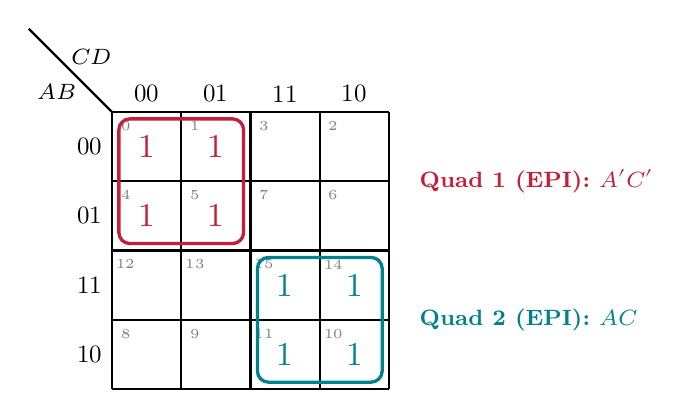
\begin{tikzpicture}[scale=0.88]
  % Grid
  \draw[thick] (0,0) grid (4,4);
  \draw[thick] (0,4) -- (-1.2, 5.2);
  \node[font=\footnotesize\bfseries] at (-0.8, 4.3) {$AB$};
  \node[font=\footnotesize\bfseries] at (-0.3, 4.8) {$CD$};

  % Column headers (CD)
  \node[above, font=\small] at (0.5, 4) {$00$};
  \node[above, font=\small] at (1.5, 4) {$01$};
  \node[above, font=\small] at (2.5, 4) {$11$};
  \node[above, font=\small] at (3.5, 4) {$10$};

  % Row headers (AB)
  \node[left, font=\small] at (0, 3.5) {$00$};
  \node[left, font=\small] at (0, 2.5) {$01$};
  \node[left, font=\small] at (0, 1.5) {$11$};
  \node[left, font=\small] at (0, 0.5) {$10$};

  % Minterm indices (gray)
  \node[font=\tiny\color{gray}] at (0.2, 3.8) {$0$};
  \node[font=\tiny\color{gray}] at (1.2, 3.8) {$1$};
  \node[font=\tiny\color{gray}] at (2.2, 3.8) {$3$};
  \node[font=\tiny\color{gray}] at (3.2, 3.8) {$2$};

  \node[font=\tiny\color{gray}] at (0.2, 2.8) {$4$};
  \node[font=\tiny\color{gray}] at (1.2, 2.8) {$5$};
  \node[font=\tiny\color{gray}] at (2.2, 2.8) {$7$};
  \node[font=\tiny\color{gray}] at (3.2, 2.8) {$6$};

  \node[font=\tiny\color{gray}] at (0.2, 1.8) {$12$};
  \node[font=\tiny\color{gray}] at (1.2, 1.8) {$13$};
  \node[font=\tiny\color{gray}] at (2.2, 1.8) {$15$};
  \node[font=\tiny\color{gray}] at (3.2, 1.8) {$14$};

  \node[font=\tiny\color{gray}] at (0.2, 0.8) {$8$};
  \node[font=\tiny\color{gray}] at (1.2, 0.8) {$9$};
  \node[font=\tiny\color{gray}] at (2.2, 0.8) {$11$};
  \node[font=\tiny\color{gray}] at (3.2, 0.8) {$10$};

  % Example 1s
  \node[font=\large\bfseries\color{myred}] at (0.5, 3.5) {$1$};
  \node[font=\large\bfseries\color{myred}] at (1.5, 3.5) {$1$};
  \node[font=\large\bfseries\color{myred}] at (0.5, 2.5) {$1$};
  \node[font=\large\bfseries\color{myred}] at (1.5, 2.5) {$1$};

  \node[font=\large\bfseries\color{myteal}] at (2.5, 1.5) {$1$};
  \node[font=\large\bfseries\color{myteal}] at (3.5, 1.5) {$1$};
  \node[font=\large\bfseries\color{myteal}] at (2.5, 0.5) {$1$};
  \node[font=\large\bfseries\color{myteal}] at (3.5, 0.5) {$1$};

  % Grouping boxes
  \draw[very thick, rounded corners=4pt, color=myred] (0.1, 2.1) rectangle (1.9, 3.9);
  \node[right, font=\footnotesize\bfseries\color{myred}] at (4.3, 3.0) {Quad 1 (EPI): $A' C'$};

  \draw[very thick, rounded corners=4pt, color=myteal] (2.1, 0.1) rectangle (3.9, 1.9);
  \node[right, font=\footnotesize\bfseries\color{myteal}] at (4.3, 1.0) {Quad 2 (EPI): $A C$};
\end{tikzpicture}
\end{tcolorbox}

\subsection{Static Hazards in Combinational Logic}
A \textbf{static hazard} is a transient unwanted glitch ($0 \to 1 \to 0$ for static-0 or $1 \to 0 \to 1$ for static-1) occurring at the output due to unequal propagation delays along converging signal paths.
\begin{itemize}[leftmargin=*, itemsep=3pt]
  \item \textbf{Cause:} A single variable changes state and transitions between two adjacent K-map prime implicant loops without an overlapping product term.
  \item \textbf{Elimination:} Add redundant consensus prime implicants to bridge adjacent loops in the K-map.
\end{itemize}

% ===============================================================================
\section{Binary Codes and Code Converters}
% ===============================================================================

Digital systems employ specialized binary codes tailored for arithmetic, display, communication, and mechanical position sensing:

\subsection{Standard Binary Codes}
\begin{itemize}[leftmargin=*, itemsep=3pt]
  \item \textbf{BCD (Binary Coded Decimal / 8421):} Each decimal digit ($0\text{--}9$) is encoded as a 4-bit binary group ($0000$ to $1001$). The six combinations $1010_2$ to $1111_2$ are invalid.
  \item \textbf{Excess-3 Code:} Unweighted, self-complementing code formed by adding $0011_2$ ($+3$) to the 8421 BCD code. The 1's complement of an Excess-3 number represents the 9's complement of its decimal equivalent.
  \item \textbf{Gray Code (Reflected Binary Unit-Distance Code):} Successive code words differ in only a single bit position ($\Delta = 1$), eliminating spurious switching errors in optical shaft encoders.
\end{itemize}

\subsection{Binary to Gray and Gray to Binary Code Conversion}
\begin{tcolorbox}[formulabox, title={\textbf{Code Conversion Logic}}]
Binary to Gray conversion ($B = b_{n-1} \dots b_0 \to G = g_{n-1} \dots g_0$):
\begin{equation}
  g_{n-1} = b_{n-1}, \qquad g_i = b_{i+1} \oplus b_i \quad (\text{for } i = 0, 1, \dots, n-2)
\end{equation}
Gray to Binary conversion ($G = g_{n-1} \dots g_0 \to B = b_{n-1} \dots b_0$):
\begin{equation}
  b_{n-1} = g_{n-1}, \qquad b_i = b_{i+1} \oplus g_i \quad (\text{for } i = 0, 1, \dots, n-2)
\end{equation}
\end{tcolorbox}

% ===============================================================================
\section{Combinational Arithmetic Circuits}
% ===============================================================================

\subsection{Half Adder, Full Adder, and Subtractors}
\par\vspace{6pt}\noindent
\begingroup
\setlength{\tabcolsep}{4pt}
\setlength{\extrarowheight}{3pt}
\renewcommand{\arraystretch}{1.35}
\begin{tabularx}{\linewidth}{|B{2.8cm}|Y|Y|}
\hline
\textbf{Circuit} & \textbf{Boolean Sum / Difference ($S, D$)} & \textbf{Carry / Borrow ($C, B$)} \\
\hline
Half Adder (HA) & $S = A \oplus B$ & $C = A \cdot B$ \\
\hline
Half Subtractor (HS) & $D = A \oplus B$ & $B_{\text{out}} = A' \cdot B$ \\
\hline
Full Adder (FA) & $S = A \oplus B \oplus C_{\text{in}}$ & $C_{\text{out}} = A B + (A \oplus B) C_{\text{in}} = A B + B C_{\text{in}} + A C_{\text{in}}$ \\
\hline
Full Subtractor (FS) & $D = A \oplus B \oplus B_{\text{in}}$ & $B_{\text{out}} = A' B + (A \oplus B)' B_{\text{in}} = A' B + A' B_{\text{in}} + B B_{\text{in}}$ \\
\hline
\end{tabularx}
\endgroup

\subsection{Ripple Carry Adder vs. Carry Lookahead Adder (CLA)}
An $n$-bit \textbf{Ripple Carry Adder (RCA)} cascades $n$ Full Adders. The carry out of stage $i$ ripples to the carry input of stage $i+1$. Total worst-case propagation delay is linear:
\begin{equation}
  t_{\text{RCA}} = 2 t_{\text{gate}} + (n-1) 2 t_{\text{gate}} = 2 n \, t_{\text{gate}}
\end{equation}
To eliminate rippling delay, the \textbf{Carry Lookahead Adder (CLA)} precomputes all stage carries in parallel using Carry Generate ($G_i$) and Carry Propagate ($P_i$) functions:
\begin{equation}
  G_i = A_i \cdot B_i, \qquad P_i = A_i \oplus B_i
\end{equation}
Expanding the stage carry expressions recursively:
\begin{align}
  C_1 &= G_0 + P_0 C_0 \\
  C_2 &= G_1 + P_1 C_1 = G_1 + P_1 G_0 + P_1 P_0 C_0 \\
  C_3 &= G_2 + P_2 G_1 + P_2 P_1 G_0 + P_2 P_1 P_0 C_0 \\
  C_4 &= G_3 + P_3 G_2 + P_3 P_2 G_1 + P_3 P_2 P_1 G_0 + P_3 P_2 P_1 P_0 C_0
\end{align}

\begin{tcolorbox}[tikzbox, title={Carry Lookahead Generator Architecture (4-bit CLA)}]
\centering
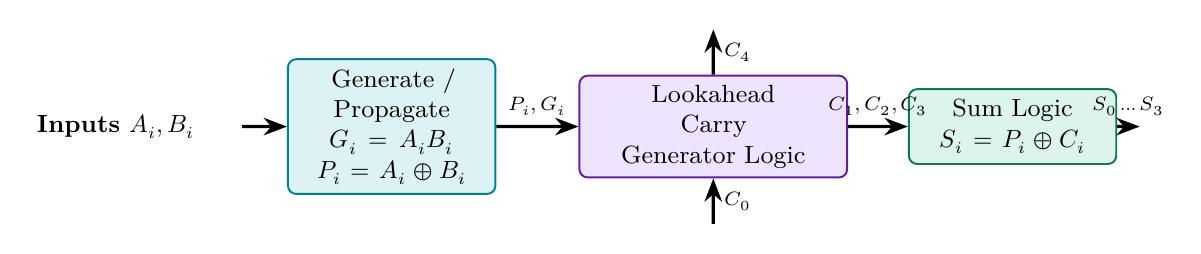
\begin{tikzpicture}[scale=0.95]
  % Inputs
  \node[left, font=\small\bfseries] at (0, 2.5) {Inputs $A_i, B_i$};
  \node[block, fill=hdrteal, draw=myteal] (gp) at (2.5, 2.5) {Generate / Propagate\\$G_i = A_i B_i$\\$P_i = A_i \oplus B_i$};

  \node[block, fill=hdrpurple, draw=mypurple, minimum width=3.4cm] (clg) at (6.8, 2.5) {Lookahead Carry\\Generator Logic};

  \node[block, fill=hdrgreen, draw=mygreen] (sum) at (10.8, 2.5) {Sum Logic\\$S_i = P_i \oplus C_i$};

  \draw[-Stealth, very thick] (0.5, 2.5) -- (gp);
  \draw[-Stealth, very thick] (gp) -- (clg) node[midway, above, font=\scriptsize] {$P_i, G_i$};
  \draw[-Stealth, very thick] (clg) -- (sum) node[midway, above, font=\scriptsize] {$C_1, C_2, C_3$};
  \draw[-Stealth, very thick] (6.8, 1.2) -- (clg) node[midway, right, font=\scriptsize] {$C_0$};
  \draw[-Stealth, very thick] (clg) -- (6.8, 3.8) node[midway, right, font=\scriptsize] {$C_4$};
  \draw[-Stealth, very thick] (sum) -- (12.5, 2.5) node[midway, above, font=\scriptsize] {$S_0 \dots S_3$};
\end{tikzpicture}
\end{tcolorbox}
\textbf{Delay Comparison:} All carries $C_1, \dots, C_4$ are generated in only $2 t_{\text{gate}}$ delays, and the final sums in $4 t_{\text{gate}}$ delays, completely independent of word length $n$.

\subsection{BCD Adder}
Adding two 4-bit BCD digits produces a sum $S_3 S_2 S_1 S_0$ and carry $K$. When the sum exceeds $9$ ($1001_2$) or a carry $K=1$ is generated, the result is an invalid BCD digit. Correction is achieved by adding $6$ ($0110_2$):
\begin{equation}
  \text{Correction Flag } C_{\text{out}} = K + S_3 S_2 + S_3 S_1
\end{equation}

% ===============================================================================
\section{MSI Combinational Logic Devices}
% ===============================================================================

\subsection{Magnitude Comparators}
A magnitude comparator compares two $n$-bit binary numbers $A = a_{n-1} \dots a_0$ and $B = b_{n-1} \dots b_0$ and asserts one of three output lines: $A > B$, $A = B$, or $A < B$.
\begin{itemize}[leftmargin=*, itemsep=3pt]
  \item Equality condition: $A = B \implies x_i = (a_i \oplus b_i)'$ for all $i$, so $(A=B) = x_{n-1} x_{n-2} \dots x_0$.
  \item Greater-than condition:
  \begin{equation}
    (A > B) = a_{n-1} b_{n-1}' + x_{n-1} a_{n-2} b_{n-2}' + \dots + x_{n-1} \dots x_1 a_0 b_0'
  \end{equation}
  \item IC 7485 is a 4-bit magnitude comparator equipped with cascading inputs ($I_{A>B}, I_{A=B}, I_{A<B}$) enabling expansion to compare 8-bit, 16-bit, or larger words.
\end{itemize}

\subsection{Multiplexers (Data Selectors)}
A multiplexer routes one of $2^n$ data input channels to a single output line under the control of $n$ selection lines:
\begin{equation}
  Y = \sum_{k=0}^{2^n-1} m_k \cdot D_k
\end{equation}
where $m_k$ is the minterm formed by the $n$ select lines $S_{n-1} \dots S_0$.
\begin{itemize}[leftmargin=*, itemsep=3pt]
  \item \textbf{Universal Logic Implementation:} Any Boolean function of $n$ variables can be implemented directly using a $2^{n-1}$-to-1 MUX by connecting $(n-1)$ variables to select lines and using the remaining variable ($0, 1, X, X'$) on the data inputs.
\end{itemize}

\subsection{Encoders and Decoders}
\begin{itemize}[leftmargin=*, itemsep=3pt]
  \item \textbf{Decoders ($n$-to-$2^n$):} Converts an $n$-bit binary input into one of $2^n$ active output lines (minterm generator). IC 74138 is a standard 3-to-8 decoder with active-low outputs.
  \item \textbf{Priority Encoders ($2^n$-to-$n$):} If two or more inputs are simultaneously asserted, the encoder generates the binary code corresponding to the input with the highest assigned priority (e.g., IC 74148 8-to-3 priority encoder).
\end{itemize}

\subsection{Barrel Shifters and Arithmetic Logic Units (ALUs)}
\begin{itemize}[leftmargin=*, itemsep=3pt]
  \item \textbf{Barrel Shifter:} A specialized digital crossbar circuit constructed from multiplexer arrays capable of shifting or rotating an $n$-bit data word by an arbitrary number of bit positions ($0$ to $n-1$) in a \textbf{single clock cycle}, avoiding sequential shift register clock cycles.
  \item \textbf{Arithmetic Logic Unit (IC 74181):} A 4-bit parallel multifunction processor element. Under the command of 4 function select inputs ($S_3 S_2 S_1 S_0$) and a mode control bit $M$ ($M=1 \implies$ Logic functions; $M=0 \implies$ Arithmetic functions with carry lookahead), it can perform all 16 logic operations and 16 arithmetic operations.
\end{itemize}

\newpage
% ===============================================================================
\section{Quick Revision Page}
% ===============================================================================

\begin{tcolorbox}[formulabox, title={\textbf{Key Formulas and Identities at a Glance}}]
\begin{itemize}[leftmargin=*, itemsep=2.5pt]
  \item \textbf{Signed 2's Complement Range:} $-2^{n-1} \le N \le 2^{n-1}-1$
  \item \textbf{2's Complement Overflow Condition:} $V = C_n \oplus C_{n-1}$
  \item \textbf{De Morgan's Laws:} $\overline{A \cdot B} = \overline{A} + \overline{B}, \quad \overline{A + B} = \overline{A} \cdot \overline{B}$
  \item \textbf{Binary-to-Gray Conversion:} $g_{n-1} = b_{n-1}, \quad g_i = b_{i+1} \oplus b_i$
  \item \textbf{Full Adder Sum \& Carry:} $S = A \oplus B \oplus C_{\text{in}}, \quad C_{\text{out}} = AB + (A \oplus B)C_{\text{in}}$
  \item \textbf{CLA Generate \& Propagate:} $G_i = A_i B_i, \quad P_i = A_i \oplus B_i, \quad C_{i+1} = G_i + P_i C_i$
  \item \textbf{BCD Adder Correction:} $C_{\text{out}} = K + S_3 S_2 + S_3 S_1$
  \item \textbf{Multiplexer Output Equation:} $Y = \sum_{k=0}^{2^n-1} m_k D_k$
\end{itemize}
\end{tcolorbox}

\begin{tcolorbox}[defbox, title={\textbf{One-Line Definitions}}]
\begin{itemize}[leftmargin=*, itemsep=2.5pt]
  \item \textbf{Minterm:} A canonical product term of $n$ variables that evaluates to logic $1$ for exactly one input combination.
  \item \textbf{Essential Prime Implicant (EPI):} A prime implicant rectangle containing at least one minterm that is not covered by any other prime implicant.
  \item \textbf{Static-1 Hazard:} A transient output glitch to $0$ occurring when an input change should have maintained a constant $1$ output.
  \item \textbf{Gray Code:} An unweighted, unit-distance binary code in which adjacent numbers differ by exactly one bit.
  \item \textbf{Priority Encoder:} An encoder that outputs the binary address of only the highest-priority active input line.
  \item \textbf{Barrel Shifter:} A combinational logic circuit that shifts or rotates an $n$-bit word by any specified number of bits in a single clock cycle.
\end{itemize}
\end{tcolorbox}

\begin{tcolorbox}[exambox, title={\textbf{Frequently Asked / Viva Questions}}]
\begin{enumerate}[label=\textbf{Q\arabic*.}, leftmargin=*]
  \item \Q{Why is 2's complement universally preferred over 1's complement in digital ALUs?}
    2's complement provides a single unique representation for zero ($0000_2$), eliminates the complex end-around carry addition required in 1's complement, and simplifies hardware subtraction into simple addition.
  \item \Q{How do you detect arithmetic overflow in 2's complement addition?}
    Overflow occurs when adding two numbers of identical sign results in a sum with the opposite sign. In hardware, it is detected when the carry into the sign bit differs from the carry out of the sign bit ($V = C_n \oplus C_{n-1} = 1$).
  \item \Q{What is the difference between Prime Implicants and Essential Prime Implicants in a K-map?}
    A Prime Implicant is a maximal group of adjacent $1$s that cannot be doubled in size. An Essential Prime Implicant is a prime implicant that covers at least one $1$ that is not covered by any other prime implicant.
  \item \Q{Explain the cause and remedy of a static-1 hazard.}
    It is caused by unequal propagation delays when a variable and its complement change simultaneously across two separate K-map loops. It is remedied by adding an extra overlapping consensus prime implicant to cover the transition.
  \item \Q{Why is Gray code extensively used in optical shaft encoders?}
    Because only a single bit changes between any two consecutive values ($\Delta = 1$), avoiding erroneous transient readings caused by mechanical switch misalignment.
  \item \Q{Why is a Carry Lookahead Adder (CLA) faster than a Ripple Carry Adder (RCA)?}
    In an RCA, carry must propagate sequentially through all $n$ stages ($t \propto n$). In a CLA, carries are computed simultaneously in two gate delays using carry generate ($G_i$) and propagate ($P_i$) logic ($t = O(1)$).
  \item \Q{What is the correction condition in a BCD adder?}
    When the binary sum of two BCD digits exceeds $9$ ($1001_2$) or generates an output carry $K=1$, the correction logic $C = K + S_3 S_2 + S_3 S_1$ adds $+6$ ($0110_2$) to skip the 6 invalid 4-bit states.
  \item \Q{How can an $n$-variable Boolean function be implemented using an $2^{n-1}$-to-1 MUX?}
    Connect $(n-1)$ variables to the select lines, and connect the data input lines to $0, 1$, or the remaining variable $X$ or $X'$ derived from a truth table partition.
  \item \Q{What is a Priority Encoder and where is it used?}
    It is an encoder that produces the binary code corresponding to the highest-order active input when multiple inputs are asserted. It is widely used in microprocessor interrupt request handling.
  \item \Q{What is the function of the mode control bit $M$ in the 74181 ALU?}
    $M=1$ disables internal carry propagation, configuring the ALU for 16 logic operations. $M=0$ enables carries, configuring the ALU for 16 arithmetic operations.
  \item \Q{Differentiate between canonical and standard Boolean expressions.}
    In canonical form (canonical SOP/POS), every individual product/sum term must contain all variables of the function. In standard form, terms may contain any subset of variables.
  \item \Q{What is a barrel shifter and why is it preferred over a shift register in microprocessors?}
    A barrel shifter uses multiplexer matrices to shift or rotate an $n$-bit word by $k$ positions in a single clock cycle, whereas an ordinary shift register requires $k$ separate clock cycles.
\end{enumerate}
\end{tcolorbox}

\begin{tcolorbox}[tikzbox, title={Comparison of Combinational MSI Building Blocks}]
\centering
\begingroup
\footnotesize
\setlength{\tabcolsep}{3.5pt}
\setlength{\extrarowheight}{2.5pt}
\renewcommand{\arraystretch}{1.35}
\begin{tabularx}{\linewidth}{|B{2.4cm}|Y|Y|Y|}
\hline
\textbf{Device} & \textbf{Input / Output Ratio} & \textbf{Control Signals} & \textbf{Primary Application} \\
\hline
Multiplexer (MUX) & $2^n$ Data Inputs $\to$ $1$ Output & $n$ Select Lines, Enable & Data routing, parallel-to-serial conversion, Boolean function synthesis \\
\hline
Demultiplexer (DEMUX) & $1$ Data Input $\to$ $2^n$ Outputs & $n$ Select Lines, Enable & Serial-to-parallel distribution, memory addressing \\
\hline
Decoder & $n$ Inputs $\to$ $2^n$ Outputs & Enable / Chip Select & Memory address decoding, 7-segment displays, minterm generation \\
\hline
Priority Encoder & $2^n$ Inputs $\to$ $n$ Outputs & Enable, Group Select & Interrupt arbitration, ADC flash encoding \\
\hline
Magnitude Comparator & $2 \times n$ Bit Inputs $\to$ $3$ Outputs & Cascading Inputs ($>, =, <$) & Arithmetic sorting, threshold checking, address limit checks \\
\hline
\end{tabularx}
\endgroup
\end{tcolorbox}


% -- Module 2 -----------------------------------------------------------------
\modulestart{2}{Latches and Flip-Flops}

\section{Latches and Flip-Flops}
% ===============================================================================

In sequential logic circuits, outputs depend not only on current inputs but also on past history stored in memory elements.

\subsection{Latches vs. Flip-Flops}
\begin{itemize}[leftmargin=*, itemsep=3pt]
  \item \textbf{Latch:} A level-triggered bistable storage device that responds continuously to inputs whenever the enable/clock signal is at an active level (transparent).
  \item \textbf{Flip-Flop:} An edge-triggered storage device that samples inputs and updates outputs only at a discrete transition (positive rising edge $\uparrow$ or negative falling edge $\downarrow$) of the clock signal.
  \item \textbf{Setup Time ($t_s$):} The minimum time for which the data input must remain stable \textit{before} the arrival of the active clock edge.
  \item \textbf{Hold Time ($t_h$):} The minimum time for which the data input must remain stable \textit{after} the active clock edge.
  \item \textbf{Metastability:} An unstable intermediate output voltage state occurring if setup or hold times are violated.
\end{itemize}

\subsection{The S-R Latch and Forbidden State}
An S-R (Set-Reset) latch constructed with cross-coupled NOR gates operates as follows:
\begin{itemize}[leftmargin=*, itemsep=3pt]
  \item $S=0, R=0 \implies Q_{n+1} = Q_n$ (No change / Hold state).
  \item $S=0, R=1 \implies Q_{n+1} = 0, \overline{Q}_{n+1} = 1$ (Reset state).
  \item $S=1, R=0 \implies Q_{n+1} = 1, \overline{Q}_{n+1} = 0$ (Set state).
  \item $S=1, R=1 \implies Q = \overline{Q} = 0$ (\textbf{Invalid / Forbidden State}). When both inputs simultaneously drop from $1$ to $0$, the circuit enters a race condition, settling into an unpredictable state.
\end{itemize}

\subsection{J-K Flip-Flop and the Race-Around Condition}
The J-K flip-flop eliminates the invalid state of the S-R flip-flop by feeding back outputs $Q$ and $\overline{Q}$ to the input AND gates:
\begin{equation}
  S = J \cdot \overline{Q}, \qquad R = K \cdot Q
\end{equation}
When $J = K = 1$, the flip-flop toggles its output on each active clock: $Q_{n+1} = \overline{Q}_n$.

\begin{tcolorbox}[defbox, title={\textbf{The Race-Around Condition in Level-Triggered JK Flip-Flops}}]
\textbf{Definition:} In a level-triggered JK flip-flop, when $J = K = 1$ and the clock pulse width $t_w$ is greater than the propagation delay $t_{pd}$ of the flip-flop ($t_{pd} < t_w$), the output toggles repeatedly and uncontrollably back and forth ($0 \to 1 \to 0 \to 1 \dots$) during the single high clock interval. At the end of the clock pulse, the final state of $Q$ is indeterminate.

\textbf{Mathematical Condition for Race-Around:}
\begin{equation}
  t_{pd} < t_w < \frac{T}{2}
\end{equation}
where $T$ is the clock period and $t_w$ is the pulse duration.

\textbf{Methods to Prevent Race-Around:}
\begin{enumerate}[label=\alph*., leftmargin=*]
  \item \textbf{Edge Triggering:} Design the circuit to respond only to steep clock transitions ($t_w \approx 0$).
  \item \textbf{Propagation Delay Control:} Choose components such that $t_{pd} > t_w$ (difficult and limits maximum operating frequency).
  \item \textbf{Master-Slave JK Flip-Flop Configuration:} The universal and standard architecture.
\end{enumerate}
\end{tcolorbox}

\subsection{Master-Slave JK Flip-Flop Architecture}
The Master-Slave JK flip-flop consists of two cascaded latches clocked on complementary phases:
\begin{itemize}[leftmargin=*, itemsep=3pt]
  \item \textbf{Master Latch:} Enabled when $\text{CLK} = 1$. It samples inputs $J$ and $K$ and updates its intermediate state ($Q_M$). The Slave latch remains disabled (isolated) because $\overline{\text{CLK}} = 0$.
  \item \textbf{Slave Latch:} When the clock falls ($\text{CLK} = 0 \implies \overline{\text{CLK}} = 1$), the Master is disabled, locking its state. The Slave is enabled and copies the state $Q_M$ to the final external output $Q$.
  \item Because the output $Q$ updates only on the clock falling edge when the Master is completely disabled, feedback cannot affect the Master during the same clock cycle, \textbf{completely eliminating race-around}.
\end{itemize}

\begin{tcolorbox}[tikzbox, title={Master-Slave JK Flip-Flop Functional Architecture}]
\centering
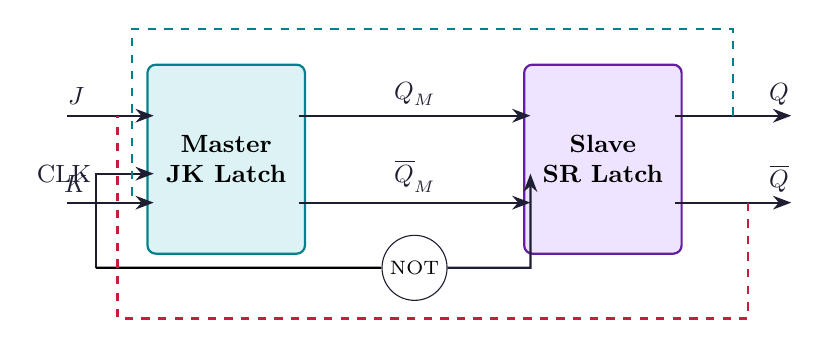
\begin{tikzpicture}[scale=0.92]
  % Master Box
  \node[ffblock, draw=myteal, fill=hdrteal] (master) at (0, 0) {Master\\JK Latch};
  % Inverter
  \node[draw=mydark, circle, inner sep=2pt, font=\scriptsize] (inv) at (2.6, -1.5) {$\text{NOT}$};
  % Slave Box
  \node[ffblock, draw=mypurple, fill=hdrpurple] (slave) at (5.2, 0) {Slave\\SR Latch};

  % Inputs
  \draw[flowarrow] (-2.2, 0.6) -- (-1.0, 0.6) node[pos=0.1, above, font=\small] {$J$};
  \draw[flowarrow] (-2.2, -0.6) -- (-1.0, -0.6) node[pos=0.1, above, font=\small] {$K$};

  % Clock distribution
  \draw[flowarrow] (-1.8, -1.5) -- (-1.8, -0.2) -- (-1.0, -0.2) node[pos=0.1, left, font=\small] {$\text{CLK}$};
  \draw[thick] (-1.8, -1.5) -- (inv);
  \draw[flowarrow] (inv) -- (4.2, -1.5) -- (4.2, -0.2);

  % Interconnect
  \draw[flowarrow] (1.0, 0.6) -- (4.2, 0.6) node[midway, above, font=\small] {$Q_M$};
  \draw[flowarrow] (1.0, -0.6) -- (4.2, -0.6) node[midway, above, font=\small] {$\overline{Q}_M$};

  % Outputs
  \draw[flowarrow] (6.2, 0.6) -- (7.8, 0.6) node[pos=0.9, above, font=\small] {$Q$};
  \draw[flowarrow] (6.2, -0.6) -- (7.8, -0.6) node[pos=0.9, above, font=\small] {$\overline{Q}$};

  % Feedback paths
  \draw[thick, dashed, color=myred] (7.2, -0.6) -- (7.2, -2.2) -- (-1.5, -2.2) -- (-1.5, 0.6);
  \draw[thick, dashed, color=myteal] (7.0, 0.6) -- (7.0, 1.8) -- (-1.3, 1.8) -- (-1.3, -0.6);
\end{tikzpicture}
\end{tcolorbox}

\subsection{Characteristic Equations and Excitation Tables}
\par\vspace{6pt}\noindent
\begingroup
\setlength{\tabcolsep}{3.5pt}
\setlength{\extrarowheight}{3pt}
\renewcommand{\arraystretch}{1.35}
\begin{tabularx}{\linewidth}{|B{1.6cm}|B{3.2cm}|Y|Y|Y|Y|}
\hline
\textbf{Type} & \textbf{Characteristic Equation} & \textbf{$Q_n \to Q_{n+1}$: $0 \to 0$} & \textbf{$0 \to 1$} & \textbf{$1 \to 0$} & \textbf{$1 \to 1$} \\
\hline
S-R & $Q_{n+1} = S + \overline{R} Q_n$ ($S R = 0$) & $S=0, R=X$ & $S=1, R=0$ & $S=0, R=1$ & $S=X, R=0$ \\
\hline
J-K & $Q_{n+1} = J \overline{Q}_n + \overline{K} Q_n$ & $J=0, K=X$ & $J=1, K=X$ & $J=X, K=1$ & $J=X, K=0$ \\
\hline
D & $Q_{n+1} = D$ & $D = 0$ & $D = 1$ & $D = 0$ & $D = 1$ \\
\hline
T & $Q_{n+1} = T \oplus Q_n$ & $T = 0$ & $T = 1$ & $T = 1$ & $T = 0$ \\
\hline
\end{tabularx}
\endgroup

% ===============================================================================
\section{Registers and Shift Registers}
% ===============================================================================

An $n$-bit register is a cascade of $n$ flip-flops sharing a common clock, designed to store and shift multi-bit binary data words.

\subsection{Shift Register Configurations}
\begin{itemize}[leftmargin=*, itemsep=3pt]
  \item \textbf{SISO (Serial-In Serial-Out):} Data enters one bit per clock cycle and exits serially. Requires $n$ clock cycles to load and $n$ clock cycles to read an $n$-bit word.
  \item \textbf{SIPO (Serial-In Parallel-Out):} Data enters serially; all $n$ bits are accessible simultaneously on parallel outputs after $n$ clock cycles.
  \item \textbf{PISO (Parallel-In Serial-Out):} Data is loaded into all flip-flops simultaneously in a single clock cycle using parallel load gates, then shifted out serially.
  \item \textbf{PIPO (Parallel-In Parallel-Out):} Parallel loading and parallel output reading simultaneously in $1$ clock cycle.
\end{itemize}

\subsection{Universal Shift Register (IC 74194)}
A bidirectional 4-bit Universal Shift Register can perform all four data transfer operations controlled by two mode select inputs $S_1, S_0$:
\begin{equation}
  S_1 S_0 = 00 \implies \text{Hold}, \quad 01 \implies \text{Shift Right}, \quad 10 \implies \text{Shift Left}, \quad 11 \implies \text{Parallel Load}
\end{equation}

% ===============================================================================
\section{Asynchronous (Ripple) and Synchronous Counters}
% ===============================================================================

A counter is a specialized sequential circuit that cycles through a prescribed sequence of binary states upon receiving clock pulses.

\subsection{Asynchronous (Ripple) Counters}
In a ripple counter, the external clock is applied \textbf{only to the first flip-flop (LSB)}. Each subsequent flip-flop is clocked by the output of the preceding stage ($Q$ or $\overline{Q}$).
\begin{itemize}[leftmargin=*, itemsep=3pt]
  \item \textbf{Up-Counter vs. Down-Counter:}
    \begin{itemize}
      \item Negative edge-triggered FF with clock connected to $Q_i \implies$ Up-counter.
      \item Negative edge-triggered FF with clock connected to $\overline{Q}_i \implies$ Down-counter.
    \end{itemize}
  \item \textbf{Mod-N Ripple Counter:} Formed by resetting all flip-flops using an active-low asynchronous clear ($\overline{\text{CLR}}$) driven by a NAND gate when the count reaches state $N$.
  \item \textbf{Disadvantages of Ripple Counters:}
    \begin{enumerate}
      \item Accumulated delay: Total propagation delay is $t_{\text{total}} = n \times t_{pd}$.
      \item Maximum operating frequency is constrained: $f_{\text{max}} \le \frac{1}{n \cdot t_{pd}}$.
      \item Transient false counting states (glitches) appear on outputs during transition intervals.
    \end{enumerate}
\end{itemize}

\subsection{Synchronous Counters}
In a synchronous counter, the master clock is connected \textbf{in parallel to all flip-flops simultaneously}. State transitions occur at the exact same clock instant.

\textbf{Systematic Synchronous Counter Design Procedure:}
\begin{enumerate}[label=\arabic*., leftmargin=*]
  \item Determine number of flip-flops: $2^n \ge N$.
  \item Construct the State Transition Diagram and State Table.
  \item Substitute flip-flop excitation requirements ($J_i, K_i$ or $T_i$ or $D_i$) from the excitation table.
  \item Minimize excitation expressions using Karnaugh maps.
  \item Implement the logic circuit.
\end{enumerate}

\subsection{Ring Counter and Johnson (Twisted Ring) Counter}
\begin{itemize}[leftmargin=*, itemsep=3pt]
  \item \textbf{Ring Counter:} An $n$-bit shift register with true output $Q_n$ fed back to serial input $D_1$. A single circulating '1' ($1000 \to 0100 \to 0010 \to 0001$).
    \begin{equation}
      \text{Number of unique states} = n, \qquad \text{Unused states} = 2^n - n
    \end{equation}
  \item \textbf{Johnson (Twisted Ring) Counter:} An $n$-bit shift register with inverted output $\overline{Q}_n$ fed back to $D_1$.
    \begin{equation}
      \text{Number of unique states} = 2n, \qquad \text{Unused states} = 2^n - 2n
    \end{equation}
    Requires only simple 2-input AND gates for complete glitch-free state decoding.
\end{itemize}

% ===============================================================================
\section{Finite State Machines (FSM)}
% ===============================================================================

Any synchronous sequential circuit can be modeled formally as a Finite State Machine consisting of combinational logic and state memory registers.

\subsection{Mealy vs. Moore FSM Models}
\begin{tcolorbox}[defbox, title={\textbf{Architectural Definitions of Mealy and Moore Machines}}]
\begin{itemize}[leftmargin=*, itemsep=3pt]
  \item \textbf{Moore Machine:} The output $Z$ depends \textbf{only on the present state} $S$:
  \begin{equation}
    Z(t) = \lambda(S(t))
  \end{equation}
  Outputs are synchronous with the clock and immune to input glitches.
  \item \textbf{Mealy Machine:} The output $Z$ depends on \textbf{both the present state $S$ and current inputs $X$}:
  \begin{equation}
    Z(t) = \lambda(S(t), X(t))
  \end{equation}
  Outputs change asynchronously as soon as inputs change, enabling faster response and generally requiring fewer states ($1$ state fewer than Moore).
\end{itemize}
\end{tcolorbox}

\begin{tcolorbox}[tikzbox, title={Block Diagrams: Moore Machine vs. Mealy Machine}]
\centering
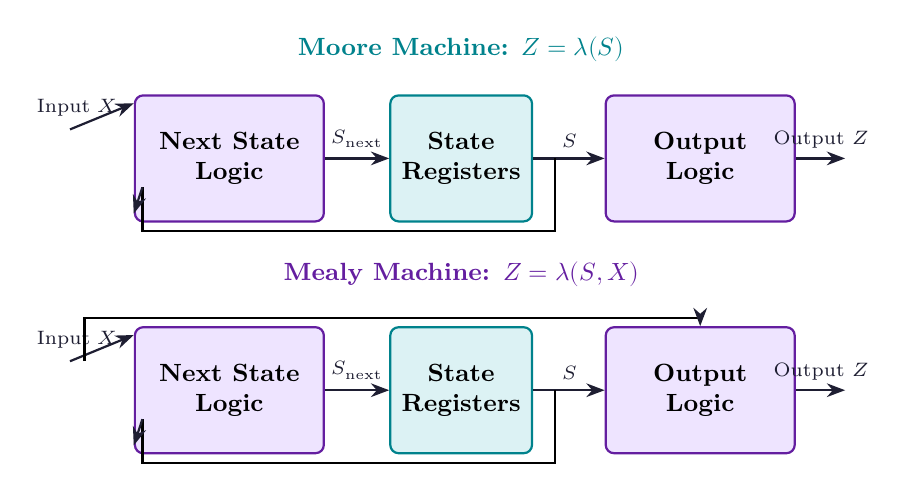
\begin{tikzpicture}[scale=0.92]
  % Moore Machine
  \begin{scope}[yshift=3.2cm]
    \node[combblock] (nsm) at (0,0) {Next State\\Logic};
    \node[ffblock, minimum width=1.8cm, minimum height=1.6cm] (regm) at (3.2,0) {State\\Registers};
    \node[combblock] (outm) at (6.5,0) {Output\\Logic};

    \draw[flowarrow] (-2.2, 0.4) -- (nsm.150) node[pos=0.1, above, font=\scriptsize] {Input $X$};
    \draw[flowarrow] (nsm) -- (regm) node[midway, above, font=\scriptsize] {$S_{\text{next}}$};
    \draw[flowarrow] (regm) -- (outm) node[midway, above, font=\scriptsize] {$S$};
    \draw[flowarrow] (outm) -- (8.5, 0) node[midway, above, font=\scriptsize] {Output $Z$};

    % Feedback
    \draw[thick] (4.5, 0) -- (4.5, -1.0) -- (-1.2, -1.0) -- (-1.2, -0.4);
    \draw[flowarrow] (-1.2, -0.4) -- (nsm.210);

    \node[above, font=\small\bfseries\color{myteal}] at (3.2, 1.2) {Moore Machine: $Z = \lambda(S)$};
  \end{scope}

  % Mealy Machine
  \begin{scope}[yshift=0cm]
    \node[combblock] (nsmy) at (0,0) {Next State\\Logic};
    \node[ffblock, minimum width=1.8cm, minimum height=1.6cm] (regmy) at (3.2,0) {State\\Registers};
    \node[combblock] (outmy) at (6.5,0) {Output\\Logic};

    \draw[flowarrow] (-2.2, 0.4) -- (nsmy.150) node[pos=0.1, above, font=\scriptsize] {Input $X$};
    \draw[flowarrow] (nsmy) -- (regmy) node[midway, above, font=\scriptsize] {$S_{\text{next}}$};
    \draw[flowarrow] (regmy) -- (outmy) node[midway, above, font=\scriptsize] {$S$};
    \draw[flowarrow] (outmy) -- (8.5, 0) node[midway, above, font=\scriptsize] {Output $Z$};

    % Input direct to output logic
    \draw[thick] (-2.0, 0.4) -- (-2.0, 1.0) -- (6.5, 1.0);
    \draw[flowarrow] (6.5, 1.0) -- (outmy.90);

    % Feedback
    \draw[thick] (4.5, 0) -- (4.5, -1.0) -- (-1.2, -1.0) -- (-1.2, -0.4);
    \draw[flowarrow] (-1.2, -0.4) -- (nsmy.210);

    \node[above, font=\small\bfseries\color{mypurple}] at (3.2, 1.3) {Mealy Machine: $Z = \lambda(S, X)$};
  \end{scope}
\end{tikzpicture}
\end{tcolorbox}

\subsection{State Reduction and State Assignment}
\begin{itemize}[leftmargin=*, itemsep=3pt]
  \item \textbf{Equivalent States:} Two states $S_1$ and $S_2$ are equivalent if for every possible input sequence, they produce identical outputs and transition to identical (or equivalent) next states.
  \item \textbf{State Reduction:} Performed using row elimination or the \textbf{Implication Table method} to eliminate redundant states, directly minimizing flip-flop count.
  \item \textbf{State Assignment Techniques:}
    \begin{itemize}
      \item \textbf{Binary Encoding:} Uses minimum number of flip-flops ($n = \lceil\log_2 N\rceil$), requires more combinational decode logic.
      \item \textbf{Gray Encoding:} Consecutive states differ by $1$ bit, minimizing switching noise and power.
      \item \textbf{One-Hot Encoding:} Uses $1$ flip-flop per state ($N$ flip-flops for $N$ states). Maximizes speed and simplifies next-state decode logic; standard choice in FPGA designs.
    \end{itemize}
\end{itemize}

% ===============================================================================
\section{Design of Synchronous Circuits}
% ===============================================================================

\subsection{Sequence Detector / Pulse Train Generator}
A sequence detector inspects an incoming serial binary bit stream and asserts output $Z = 1$ whenever a specific target pattern (e.g., $1011$) is recognized.
\begin{itemize}[leftmargin=*, itemsep=3pt]
  \item \textbf{Overlapping Sequence Detection:} The final bit(s) of a detected sequence can serve as the prefix of the next sequence. For $1011$ with input $1011011 \dots$, two detections occur.
  \item \textbf{Non-Overlapping Sequence Detection:} The detector resets to the initial state upon finding the sequence; subsequent detection starts afresh.
\end{itemize}

\subsection{Pseudo-Random Binary Sequence (PRBS) Generator}
A PRBS generator produces a deterministic, periodic binary sequence possessing noise-like statistical properties using a \textbf{Linear Feedback Shift Register (LFSR)}.
\begin{itemize}[leftmargin=*, itemsep=3pt]
  \item Constructed from an $n$-stage shift register where the input to the first flip-flop is the XOR sum of specific tap outputs defined by a primitive polynomial:
  \begin{equation}
    P(X) = X^n + c_{n-1} X^{n-1} + \dots + c_1 X + 1
  \end{equation}
  \item \textbf{Maximal-Length Sequence (m-sequence):} When $P(X)$ is primitive, the LFSR cycles through all possible non-zero states:
  \begin{equation}
    L = 2^n - 1
  \end{equation}
  (The all-zero state $00 \dots 0$ must be avoided because $\text{XOR}(0,0) = 0$, causing lock-up).
  \item \textbf{Key Applications:} Spread-spectrum communications (CDMA PN codes), cryptographic stream ciphers, and Built-In Self-Test (BIST) pseudo-random test pattern generators.
\end{itemize}

\newpage
% ===============================================================================
\section{Quick Revision Page}
% ===============================================================================

\begin{tcolorbox}[formulabox, title={\textbf{Key Sequential Formulas and Equations at a Glance}}]
\begin{itemize}[leftmargin=*, itemsep=2.5pt]
  \item \textbf{SR Flip-Flop Equation:} $Q_{n+1} = S + \overline{R} Q_n \quad (S \cdot R = 0)$
  \item \textbf{JK Flip-Flop Equation:} $Q_{n+1} = J \overline{Q}_n + \overline{K} Q_n$
  \item \textbf{D Flip-Flop Equation:} $Q_{n+1} = D$
  \item \textbf{T Flip-Flop Equation:} $Q_{n+1} = T \oplus Q_n$
  \item \textbf{Race-Around Condition:} $t_{pd} < t_w < T/2 \quad (J=K=1)$
  \item \textbf{Ripple Counter Maximum Delay:} $t_{\text{total}} = n \cdot t_{pd} \implies f_{\text{max}} = 1/(n \cdot t_{pd})$
  \item \textbf{Ring Counter States:} $N = n \quad (n\text{-bit shift register})$
  \item \textbf{Johnson Counter States:} $N = 2n \quad (n\text{-bit shift register})$
  \item \textbf{Maximal LFSR / PRBS Period:} $L = 2^n - 1$
\end{itemize}
\end{tcolorbox}

\begin{tcolorbox}[defbox, title={\textbf{One-Line Definitions}}]
\begin{itemize}[leftmargin=*, itemsep=2.5pt]
  \item \textbf{Setup Time ($t_s$):} Minimum interval data must remain stable before the active clock edge.
  \item \textbf{Hold Time ($t_h$):} Minimum interval data must remain stable after the active clock edge.
  \item \textbf{Race-Around Condition:} Repeated uncontrolled toggling of a level-triggered JK flip-flop during clock high when $t_{pd} < t_w$.
  \item \textbf{Moore Machine:} A finite state machine whose output is strictly a function of current state only.
  \item \textbf{Mealy Machine:} A finite state machine whose output depends simultaneously on current state and current inputs.
  \item \textbf{Johnson Counter:} An inverted feedback shift register producing $2n$ states for $n$ flip-flops.
\end{itemize}
\end{tcolorbox}

\begin{tcolorbox}[exambox, title={\textbf{Frequently Asked / Viva Questions}}]
\begin{enumerate}[label=\textbf{Q\arabic*.}, leftmargin=*]
  \item \Q{What is the difference between a latch and a flip-flop?}
    A latch is level-triggered (transparent whenever clock/enable is active), whereas a flip-flop is edge-triggered (samples and locks data strictly on clock transition edges).
  \item \Q{Explain the race-around condition in a JK flip-flop. How is it eliminated?}
    When $J=K=1$ in a level-triggered JK FF, if pulse width $t_w > t_{pd}$, the output toggles multiple times before the clock drops, leaving an uncertain final state. It is eliminated by using edge triggering or a Master-Slave configuration.
  \item \Q{Why is Master-Slave JK flip-flop pulse-triggered rather than edge-triggered?}
    Because the master accepts data while the clock is high, and data transfers to the slave on the falling edge; output changes only once per complete clock period.
  \item \Q{How do you convert a JK flip-flop into a D flip-flop?}
    Connect input $D$ directly to $J$, and connect an inverted $D$ ($\overline{D}$) to $K$ ($J = D, K = \overline{D}$).
  \item \Q{What is the propagation delay limitation of ripple counters?}
    Carries must ripple through each stage sequentially ($t = n \cdot t_{pd}$), which limits the maximum clock frequency and creates transient false decoding spikes (glitches).
  \item \Q{Compare Ring counter and Johnson counter for an $n$-bit shift register.}
    A ring counter yields $n$ states and requires no decoding gates. A Johnson counter yields $2n$ states and requires simple 2-input AND gates for decoding.
  \item \Q{What are the key architectural differences between Mealy and Moore FSMs?}
    In a Moore machine, output depends solely on current state ($Z = \lambda(S)$); in a Mealy machine, output depends on both current state and inputs ($Z = \lambda(S, X)$).
  \item \Q{Why does a Mealy machine typically require fewer states than a Moore machine?}
    Because Mealy outputs can vary immediately within a state based on different inputs, whereas a Moore machine requires distinct states for distinct output combinations.
  \item \Q{What is meant by One-Hot state assignment?}
    An encoding scheme using $N$ flip-flops for $N$ states where exactly one flip-flop is high ('1') at any time. It minimizes combinational decoding delay and is optimal for FPGAs.
  \item \Q{What is an LFSR and why can the all-zero state not be used?}
    A Linear Feedback Shift Register uses XOR taps to generate pseudo-random sequences. If all flip-flops become $0$, $\text{XOR}(0,0)=0$, locking the register in permanent zeros.
  \item \Q{What is metastability in digital circuits?}
    A condition where a flip-flop's output hovers at an undefined intermediate voltage level between logic $0$ and $1$ for an indeterminate duration due to a setup/hold time violation.
  \item \Q{How does an overlapping sequence detector differ from a non-overlapping one?}
    An overlapping detector allows the trailing bits of a detected sequence to be reused as the leading bits of the subsequent sequence, producing more output pulses.
\end{enumerate}
\end{tcolorbox}

\begin{tcolorbox}[tikzbox, title={Comparison: Ripple vs. Synchronous Counters and Mealy vs. Moore FSM}]
\centering
\begingroup
\footnotesize
\setlength{\tabcolsep}{3.5pt}
\setlength{\extrarowheight}{2.5pt}
\renewcommand{\arraystretch}{1.35}
\begin{tabularx}{\linewidth}{|B{2.2cm}|Y|Y|Y|}
\hline
\textbf{Category} & \textbf{Architecture A} & \textbf{Architecture B} & \textbf{Key Design Trade-off} \\
\hline
Counter Clocking & \textbf{Ripple Counter:} Flip-flops clocked by previous output & \textbf{Synchronous Counter:} All flip-flops clocked simultaneously & Ripple uses simpler wiring but has high cumulative delay; Synchronous achieves maximum speed. \\
\hline
FSM Output Logic & \textbf{Moore Machine:} $Z = \lambda(S)$ (State only) & \textbf{Mealy Machine:} $Z = \lambda(S, X)$ (State \& Input) & Moore is glitch-free and simpler; Mealy responds 1 cycle faster with fewer states. \\
\hline
Shift Register Counting & \textbf{Ring Counter:} $N = n$ states, uncomplemented loop & \textbf{Johnson Counter:} $N = 2n$ states, inverted loop & Johnson provides double the count states with minimal decoding hardware. \\
\hline
\end{tabularx}
\endgroup
\end{tcolorbox}


% -- Module 3 -----------------------------------------------------------------
\modulestart{3}{Digital Logic Families and Performance Metrics}

\section{Digital Logic Families and Performance Metrics}
% ===============================================================================

Digital Integrated Circuits (ICs) are fabricated using distinct semiconductor device technologies categorized into bipolar and metal-oxide-semiconductor (MOS) technologies.

\subsection{Key Performance Metrics of Digital ICs}
\begin{tcolorbox}[defbox, title={\textbf{Core Figures of Merit for Logic Families}}]
\begin{itemize}[leftmargin=*, itemsep=4pt]
  \item \textbf{Propagation Delay ($t_{pd}$):} The finite time required for a signal to transition through a gate from input to output, defined as the average of low-to-high ($t_{PLH}$) and high-to-low ($t_{PHL}$) transition times measured at the $50\%$ amplitude points:
  \begin{equation}
    t_{pd} = \frac{t_{PLH} + t_{PHL}}{2}
  \end{equation}
  \item \textbf{Power Dissipation ($P_D$):} The electrical power supplied by the DC source to the gate:
  \begin{equation}
    P_D = I_{CC(\text{avg})} \times V_{CC} = \left(\frac{I_{CCH} + I_{CCL}}{2}\right) \times V_{CC}
  \end{equation}
  \item \textbf{Power-Delay Product (PDP):} The fundamental figure of merit reflecting the speed-power trade-off (expressed in Joules or picojoules, pJ):
  \begin{equation}
    \text{PDP} = P_D \times t_{pd}
  \end{equation}
  A smaller PDP denotes a superior, highly efficient logic family.

  \pagebreak

  \item \textbf{Noise Margins ($NM_H, NM_L$):} The maximum spurious noise voltage amplitude that can be superimposed on an input logic signal without corrupting the recognized output state:
  \begin{align}
    \text{High-State Noise Margin:} \quad NM_H &= V_{OH(\min)} - V_{IH(\min)} \\
    \text{Low-State Noise Margin:} \quad NM_L &= V_{IL(\max)} - V_{OL(\max)}
  \end{align}
  \item \textbf{Fan-Out ($N$):} The maximum number of standard load inputs of the same family that a gate output can reliably drive without degrading logic levels:
  \begin{equation}
    N = \min\left( \left\lfloor\frac{I_{OH(\max)}}{I_{IH(\max)}}\right\rfloor, \left\lfloor\frac{I_{OL(\max)}}{I_{IL(\max)}}\right\rfloor \right)
  \end{equation}
  \item \textbf{Fan-In:} The total number of independent physical input lines available on a logic gate.
\end{itemize}
\end{tcolorbox}

\subsection{TTL (Transistor-Transistor Logic)}
TTL uses saturated BJT switches operating at a nominal supply voltage of $V_{CC} = 5.0\text{ V}$.
\begin{itemize}[leftmargin=*, itemsep=3pt]
  \item \textbf{Multi-Emitter Input BJT ($Q_1$):} Serves as the input AND gate. When any input is LOW ($0.2\text{ V}$), $Q_1$ conducts heavily, draining base current away from the phase splitter ($Q_2$), forcing $Q_2$ and output pull-down ($Q_4$) to turn OFF.
  \item \textbf{Phase Splitter Transistor ($Q_2$):} Produces complementary collector and emitter voltages to drive the push-pull output stage.
  \item \textbf{Totem-Pole Output Stage:} Consists of an active pull-up BJT ($Q_3$), series protection diode ($D_1$), and pull-down BJT ($Q_4$).
    \begin{itemize}
      \item \textit{Advantage:} Provides active low output impedance during both transitions ($0 \to 1$ and $1 \to 0$), rapidly charging and discharging parasitic capacitive loads.
      \item \textit{Critical Rule:} \textbf{Totem-pole outputs must NEVER be tied together directly in a wire-AND configuration.} If one gate output attempts to pull HIGH while another pulls LOW, a destructive direct low-resistance short-circuit path from $V_{CC}$ to ground occurs, causing excessive current spikes and thermal destruction.
    \end{itemize}
  \item \textbf{Open-Collector (OC) TTL:} Omits internal pull-up transistor $Q_3$ and diode $D_1$, leaving the collector of $Q_4$ floating.
    \begin{itemize}
      \item An external pull-up resistor $R_P$ tied to $V_{CC}$ is required.
      \item Permits \textbf{Wired-AND} logic: Multiple OC collectors can be tied together to a single node. The node is HIGH only if all connected gates turn OFF their pull-down transistors.
      \item \textbf{Pull-Up Resistor Calculation:}
      \begin{align}
        R_{P(\max)} &= \frac{V_{CC} - V_{OH(\min)}}{n \cdot I_{OH(\text{leak})} + N \cdot I_{IH(\max)}} \\
        R_{P(\min)} &= \frac{V_{CC} - V_{OL(\max)}}{I_{OL(\max)} - N \cdot I_{IL(\max)}}
      \end{align}
    \end{itemize}
  \item \textbf{Tri-State Logic (TSL):} Features three distinct electrical output states: Logic HIGH, Logic LOW, and \textbf{High-Impedance (Hi-Z)}. When the gate is disabled, both totem-pole transistors are simultaneously turned OFF, electrically isolating the node from the shared bus.
\end{itemize}

\subsection{ECL (Emitter-Coupled Logic)}
ECL operates on a \textbf{non-saturating BJT current-steering} differential pair.
\begin{itemize}[leftmargin=*, itemsep=3pt]
  \item \textbf{Non-Saturating Operation:} Transistors operate strictly in the active and cutoff regions. By preventing BJTs from entering deep saturation, the base minority carrier storage time ($t_s$) is completely eliminated.
  \item \textbf{Speed:} Fastest bipolar family ($t_{pd} \le 1\text{ ns}$).
  \item \textbf{Power Supply:} Operates with a negative supply voltage ($V_{EE} = -5.2\text{ V}$, collector ground $V_{CC} = 0\text{ V}$) to protect noise immunity against power supply surges.
  \item \textbf{Complementary Outputs:} Provides true OR and NOR outputs simultaneously.
  \item \textbf{Disadvantages:} Extremely high continuous static power dissipation ($P_D \approx 25\text{--}40\text{ mW/gate}$); very small noise margins ($NM \approx 0.2\text{--}0.25\text{ V}$).
\end{itemize}

\subsection{CMOS Logic Family}
CMOS (Complementary Metal-Oxide-Semiconductor) circuits combine complementary pairs of enhancement-mode PMOS and NMOS transistors.
\begin{itemize}[leftmargin=*, itemsep=3pt]
  \item \textbf{Structure:} Pull-Up Network (PUN) composed of PMOS transistors connected to $V_{DD}$, and Pull-Down Network (PDN) composed of NMOS transistors connected to $V_{SS}$ (GND). For any valid input combination, exactly one network conducts while the other remains completely OFF.
  \item \textbf{CMOS Inverter VTC:} Features five regions:
    \begin{itemize}
      \item \textit{Region A ($V_{in} < V_{tn}$):} NMOS OFF, PMOS linear ($V_{out} = V_{DD}$).
      \item \textit{Region B ($V_{tn} \le V_{in} < V_{th}$):} NMOS saturated, PMOS linear.
      \item \textit{Region C ($V_{in} = V_{th}$):} Both NMOS and PMOS in saturation (steepest transition).
      \item \textit{Region D ($V_{th} < V_{in} \le V_{DD} - |V_{tp}|$):} NMOS linear, PMOS saturated.
      \item \textit{Region E ($V_{in} > V_{DD} - |V_{tp}|$):} NMOS linear, PMOS OFF ($V_{out} = 0\text{ V}$).
    \end{itemize}
  \item \textbf{Transistor Sizing:} Because electron mobility is higher than hole mobility ($\mu_n \approx 2.5 \mu_p$), the PMOS width must be designed approximately $2.5$ times wider than the NMOS width:
  \begin{equation}
    \left(\frac{W}{L}\right)_p \approx 2.5 \left(\frac{W}{L}\right)_n \implies V_{th} = \frac{V_{DD}}{2}
  \end{equation}
  \item \textbf{Power Dissipation in CMOS:}
    \begin{itemize}
      \item \textit{Static Power:} Negligible leakage current ($I_{\text{leak}} \times V_{DD} \approx \text{nW}$).
      \item \textit{Dynamic Power:} Dominates during high-frequency switching when charging/discharging load capacitance $C_L$:
      \begin{equation}
        P_{\text{dyn}} = \alpha \cdot C_L \cdot V_{DD}^2 \cdot f
      \end{equation}
      where $\alpha$ is the switching activity factor ($0 \le \alpha \le 1$), and $f$ is clock frequency.
    \end{itemize}
  \item \textbf{CMOS Transmission Gate (TG):} A parallel combination of NMOS and PMOS controlled by complementary gating signals ($C, \overline{C}$). Passes the entire voltage range from $0$ to $V_{DD}$ without suffering threshold voltage drops ($V_{tn}, |V_{tp}|$).
\end{itemize}

\par\vspace{6pt}\noindent
\begingroup
\setlength{\tabcolsep}{3.5pt}
\setlength{\extrarowheight}{3pt}
\begin{tabularx}{\linewidth}{|B{2.2cm}|Y|Y|Y|Y|}
\hline
\textbf{Parameter} & \textbf{Standard TTL (74xx)} & \textbf{Schottky TTL (74S)} & \textbf{ECL (10K)} & \textbf{CMOS (74HC)} \\
\hline
Device Type & Bipolar (saturated) & Bipolar (Schottky clamped) & Bipolar (non-saturated) & MOSFET (CMOS) \\
\hline
Supply Voltage ($V_{CC}$) & $+5.0\text{ V} \pm 5\%$ & $+5.0\text{ V} \pm 5\%$ & $-5.2\text{ V}$ & $+2.0\text{ V}$ to $+6.0\text{ V}$ \\
\hline
Propagation Delay ($t_{pd}$) & $10\text{ ns}$ & $3\text{ ns}$ & $1\text{ ns}$ (Fastest) & $8\text{ ns}$ (at $5\text{ V}$) \\
\hline
Power Dissipation ($P_D$) & $10\text{ mW/gate}$ & $19\text{ mW/gate}$ & $25\text{--}40\text{ mW/gate}$ & $10\text{ nW}$ (Static) \\
\hline
\end{tabularx}
\endgroup

\par\vspace{6pt}\noindent
\begingroup
\setlength{\tabcolsep}{3.5pt}
\setlength{\extrarowheight}{3pt}
\begin{tabularx}{\linewidth}{|B{2.2cm}|Y|Y|Y|Y|}
\hline
\textbf{Parameter (contd.)} & \textbf{Standard TTL (74xx)} & \textbf{Schottky TTL (74S)} & \textbf{ECL (10K)} & \textbf{CMOS (74HC)} \\
\hline
Power-Delay Product & $100\text{ pJ}$ & $57\text{ pJ}$ & $25\text{--}40\text{ pJ}$ & $< 1\text{ pJ}$ (Lowest) \\
\hline
Noise Margin ($NM$) & $0.4\text{ V}$ & $0.3\text{ V}$ & $0.2\text{--}0.25\text{ V}$ & $0.3\text{--}0.45 \times V_{DD}$ (High) \\
\hline
Fan-Out & $10$ & $10$ & $25$ & $> 50$ (Static limit $\infty$) \\
\hline
\end{tabularx}
\endgroup

% ===============================================================================
\section{Semiconductor Memories}
% ===============================================================================

Semiconductor memories are organized as arrays of $2^k \times m$ bits, where $k$ is the number of address lines ($2^k$ addressable memory words) and $m$ is the data word length.

\subsection{Random Access Memory: SRAM vs. DRAM}
\begin{itemize}[leftmargin=*, itemsep=4pt]
  \item \textbf{SRAM (Static RAM):}
    \begin{itemize}
      \item \textbf{Cell Structure:} Consists of a \textbf{6-Transistor (6T) CMOS cell}. Two cross-coupled CMOS inverters form a bi-stable latch storing true ($Q$) and complementary ($\overline{Q}$) nodes, accessed via two NMOS pass transistors activated by the Word Line (WL).
      \item \textbf{Operation:} When $\text{WL} = 1$, access transistors connect storage nodes to Bit Lines ($BL$ and $\overline{BL}$). Sensed by high-speed differential sense amplifiers.
      \item \textbf{Characteristics:} Fast access times ($1\text{--}10\text{ ns}$), no periodic refresh required, retained as long as DC power is present.
      \item \textbf{Drawback:} Requires 6 transistors per bit cell; low packaging density, high silicon area, expensive. Used primarily for Level 1/2/3 CPU cache memory.
    \end{itemize}
  \item \textbf{DRAM (Dynamic RAM):}
    \begin{itemize}
      \item \textbf{Cell Structure:} Consists of a minimal \textbf{1-Transistor 1-Capacitor (1T-1C) cell}. Binary data is stored as electrostatic charge on a tiny trench or stacked MOS capacitor ($C_s \approx 20\text{--}40\text{ fF}$).
      \item \textbf{Refresh Cycle:} Sub-threshold junction leakage discharges the capacitor over time. The entire memory must be periodically read and rewritten (\textbf{refreshed every few milliseconds}) by dedicated refresh controllers.
      \item \textbf{Destructive Read:} Reading transfers the tiny capacitor charge onto the bit line capacitance, altering the stored value. Every read cycle must automatically be followed by an internal precharge and write-back restoration cycle.
      \item \textbf{Characteristics:} Highest packing density, lowest cost per bit, but slower access time ($30\text{--}60\text{ ns}$). Standard choice for computer main memory (DDR4/DDR5 SDRAM).
    \end{itemize}
\end{itemize}

\par\vspace{6pt}\noindent
\begingroup
\setlength{\tabcolsep}{3.5pt}
\setlength{\extrarowheight}{3pt}
\begin{tabularx}{\linewidth}{|B{2.8cm}|Y|Y|}
\hline
\textbf{Feature} & \textbf{Static RAM (SRAM)} & \textbf{Dynamic RAM (DRAM)} \\
\hline
Basic Storage Cell & 6 Transistors (Cross-coupled inverters) & 1 Transistor + 1 Storage Capacitor (1T-1C) \\
\hline
Storage Principle & Bi-stable latch state & Electrostatic charge on capacitor \\
\hline
Refresh Required? & No & Yes (periodically every $2\text{--}64\text{ ms}$) \\
\hline
Read Operation & Non-destructive & Destructive (requires write-back) \\
\hline
Access Speed & Extremely Fast ($1\text{--}10\text{ ns}$) & Moderate ($30\text{--}60\text{ ns}$) \\
\hline
Density / Cell Area & Low density (large cell area) & Extremely High density (minimal cell area) \\
\hline
Power Consumption & Low static, higher dynamic & Low idle, power consumed during refresh \\
\hline
Primary Applications & CPU L1/L2/L3 Cache, register files & Main system RAM (PC, servers, smartphones) \\
\hline
\end{tabularx}
\endgroup

\subsection{Read-Only Memories (ROM) and Flash Memory}
\begin{itemize}[leftmargin=*, itemsep=3pt]
  \item \textbf{Mask ROM:} Data programmed permanently during IC semiconductor fabrication using customized metallization masks. Zero reprogramming capability; economical only in vast production volumes.
  \item \textbf{PROM (Programmable ROM):} Shipped with all bits containing intact fuses or antifuses. The user permanently programs the chip using high-voltage current pulses that blow selected fuses. One-time programmable (OTP).
  \item \textbf{EPROM (Erasable PROM):} Uses Floating-Gate Avalanche-injection MOS (FAMOS) transistors. Electrons injected into isolated polysilicon floating gates alter threshold voltages. Erased completely by exposing the die to strong \textbf{Ultraviolet (UV) radiation} ($253.7\text{ nm}$) through a transparent quartz window for $15\text{--}20\text{ minutes}$. Cannot be erased in-circuit or selectively byte-erased.
  \item \textbf{EEPROM (Electrically Erasable PROM):} Utilizes Floating Gate Tunnel Oxide (FLOTOX) structures. Electrons are transferred to/from floating gates via \textbf{Fowler-Nordheim quantum mechanical tunneling}. Can be erased and rewritten electrically byte-by-byte in-circuit without UV light.
  \item \textbf{Flash Memory:} Advanced high-density EEPROM with block-level erase capability:
    \begin{itemize}
      \item \textbf{NOR Flash:} Storage cells connected in parallel. Supports random access and execute-in-place (XIP) memory architectures. Ideal for storing microcontroller firmware and BIOS code.
      \item \textbf{NAND Flash:} Storage cells connected in series strings. Provides significantly higher silicon packing density, faster write and erase cycle times, and lower cost per gigabyte. Standard technology for USB flash drives, memory cards, and Solid-State Drives (SSDs).
    \end{itemize}
\end{itemize}

% ===============================================================================
\section{Programmable Logic Devices (PLDs) and FPGAs}
% ===============================================================================

Programmable Logic Devices are standard ICs containing reconfigurable arrays of logic gates and storage elements that allow custom digital circuits to be implemented post-fabrication.

\subsection{Classification of Simple PLDs (SPLDs)}
\begin{tcolorbox}[defbox, title={\textbf{Architectural Comparison of PROM, PLA, and PAL}}]
\begin{itemize}[leftmargin=*, itemsep=4pt]
  \item \textbf{PROM as a PLD:}
    \begin{itemize}
      \item \textbf{AND Array:} Fixed (configured as a complete $k$-to-$2^k$ binary decoder generating all $2^k$ minterms).
      \item \textbf{OR Array:} Fully Programmable.
      \item \textit{Limitation:} Fixed full decoding wastes chip area when functions require only a small subset of minterms.
    \end{itemize}
  \item \textbf{PLA (Programmable Logic Array):}
    \begin{itemize}
      \item \textbf{AND Array:} Fully Programmable.
      \item \textbf{OR Array:} Fully Programmable.
      \item \textit{Advantage:} Maximum functional flexibility; allows sharing of product terms among multiple output functions.
      \item \textit{Drawback:} Higher internal propagation delay and complex programming hardware.
    \end{itemize}
  \item \textbf{PAL (Programmable Array Logic):}
    \begin{itemize}
      \item \textbf{AND Array:} Fully Programmable.
      \item \textbf{OR Array:} Fixed (each OR gate is hardwired to a predetermined set of AND gate outputs).
      \item \textit{Advantage:} Faster propagation speed, simpler fabrication, and lower cost compared to PLA.
    \end{itemize}
\end{itemize}
\end{tcolorbox}

\begin{tcolorbox}[tikzbox, title={Architectural Comparison: PROM vs. PLA vs. PAL}]
\centering
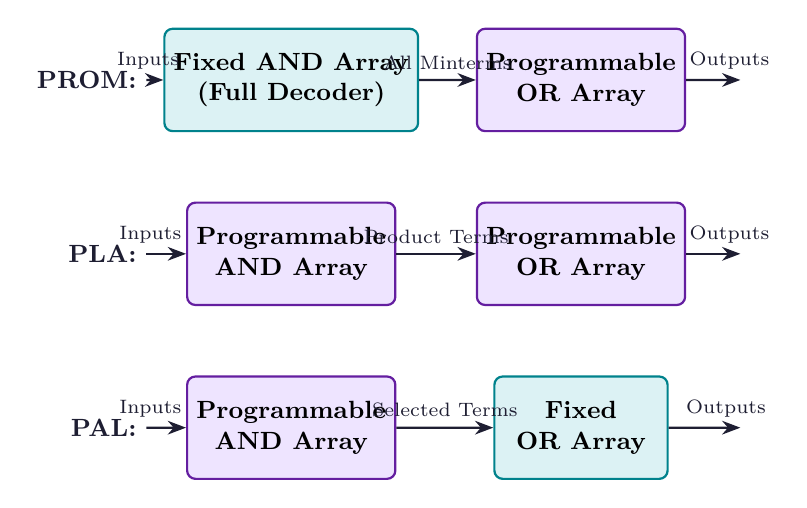
\begin{tikzpicture}[scale=0.92]
  % PROM
  \node[sysblock, draw=myteal, fill=hdrteal] (p1) at (0, 2.4) {Fixed AND Array\\(Full Decoder)};
  \node[sysblock, draw=mypurple, fill=hdrpurple] (p2) at (4.0, 2.4) {Programmable\\OR Array};
  \draw[flowarrow] (-2.0, 2.4) -- (p1) node[pos=0.1, above, font=\scriptsize] {Inputs};
  \draw[flowarrow] (p1) -- (p2) node[midway, above, font=\scriptsize] {All Minterms};
  \draw[flowarrow] (p2) -- (6.2, 2.4) node[pos=0.8, above, font=\scriptsize] {Outputs};
  \node[left, font=\small\bfseries\color{mydark}] at (-2.0, 2.4) {PROM:};

  % PLA
  \node[sysblock, draw=mypurple, fill=hdrpurple] (pa1) at (0, 0) {Programmable\\AND Array};
  \node[sysblock, draw=mypurple, fill=hdrpurple] (pa2) at (4.0, 0) {Programmable\\OR Array};
  \draw[flowarrow] (-2.0, 0) -- (pa1) node[pos=0.1, above, font=\scriptsize] {Inputs};
  \draw[flowarrow] (pa1) -- (pa2) node[midway, above, font=\scriptsize] {Product Terms};
  \draw[flowarrow] (pa2) -- (6.2, 0) node[pos=0.8, above, font=\scriptsize] {Outputs};
  \node[left, font=\small\bfseries\color{mydark}] at (-2.0, 0) {PLA:};

  % PAL
  \node[sysblock, draw=mypurple, fill=hdrpurple] (pl1) at (0, -2.4) {Programmable\\AND Array};
  \node[sysblock, draw=myteal, fill=hdrteal] (pl2) at (4.0, -2.4) {Fixed\\OR Array};
  \draw[flowarrow] (-2.0, -2.4) -- (pl1) node[pos=0.1, above, font=\scriptsize] {Inputs};
  \draw[flowarrow] (pl1) -- (pl2) node[midway, above, font=\scriptsize] {Selected Terms};
  \draw[flowarrow] (pl2) -- (6.2, -2.4) node[pos=0.8, above, font=\scriptsize] {Outputs};
  \node[left, font=\small\bfseries\color{mydark}] at (-2.0, -2.4) {PAL:};
\end{tikzpicture}
\end{tcolorbox}

\subsection{Complex Programmable Logic Devices (CPLD)}
A CPLD integrates multiple PAL/GAL-like \textbf{Function Blocks (Logic Array Blocks)} interconnected through a centralized, uniform \textbf{Global Interconnect Matrix (GIM)}.
\begin{itemize}[leftmargin=*, itemsep=3pt]
  \item Features non-volatile EEPROM/Flash configuration storage (starts up instantly upon power application).
  \item Delivers predictable, deterministic pin-to-pin propagation timing delays.
  \item Typically contains tens to hundreds of macrocells (equivalent to $1{,}000$ to $100{,}000$ logic gates).
\end{itemize}

\subsection{Field Programmable Gate Arrays (FPGA)}
FPGAs are high-density digital ICs based on an \textbf{island-style architecture} consisting of a two-dimensional matrix of programmable logic resources:
\begin{itemize}[leftmargin=*, itemsep=4pt]
  \item \textbf{Configurable Logic Blocks (CLBs):} The fundamental computational building blocks. Each CLB contains:
    \begin{itemize}
      \item \textbf{Look-Up Tables (LUTs):} A $k$-input LUT is a small high-speed SRAM block ($2^k \times 1$) that implements \textbf{any arbitrary Boolean logic function of $k$ variables} simply by loading the function's truth table truth bits into memory. The inputs serve as address lines selecting the precomputed output bit.
      \item \textbf{Storage Elements:} Configurable D flip-flops / latches with clock enables, set/reset lines.
      \item \textbf{Arithmetic Carry Logic:} Dedicated ultra-fast lookahead carry chains for high-speed addition.
      \item \textbf{Multiplexers:} Wide multiplexers for combining multiple LUT outputs.
    \end{itemize}
  \item \textbf{Programmable Interconnects:} Segmented horizontal and vertical routing channels joined at programmable \textbf{Switch Boxes} and \textbf{Connection Boxes}.
  \item \textbf{Input/Output Blocks (IOBs):} Configurable bidirectional input/output buffers surrounding the periphery, supporting multiple I/O standards (LVTTL, LVCMOS, differential signaling).
  \item \textbf{Specialized Hardware Blocks:} Modern FPGAs embed dedicated DSP slices (hardwired MAC units), dual-port block RAMs (BRAM), PLLs/DCMs, and high-speed transceivers.
\end{itemize}

\par\vspace{6pt}\noindent
\begingroup
\setlength{\tabcolsep}{3.5pt}
\setlength{\extrarowheight}{3pt}
\begin{tabularx}{\linewidth}{|B{2.8cm}|Y|Y|}
\hline
\textbf{Feature} & \textbf{CPLD} & \textbf{FPGA} \\
\hline
Architecture & Coarse-grained (PAL-like function blocks) & Fine-grained (2D array of CLBs and LUTs) \\
\hline
Configuration Memory & Non-volatile (Internal Flash/EEPROM) & Volatile (SRAM-based, requires boot ROM) \\
\hline
Boot-up Time & Instant-on upon power application & Requires configuration bitstream loading \\
\hline
Interconnect & Global interconnect matrix (Centralized) & Segmented channels and switch matrices \\
\hline
Timing Predictability & Deterministic, fixed pin-to-pin delay & Variable, placement and routing dependent \\
\hline
Density / Logic Capacity & Low to moderate ($< 10{,}000$ macrocells) & Extremely High (Millions of system gates) \\
\hline
Typical Applications & Glue logic, boot controllers, address decoders & DSP, telecommunications, AI acceleration, ASIC prototyping \\
\hline
\end{tabularx}
\endgroup

% ===============================================================================
\section{Digital-to-Analog Converters (DAC)}
% ===============================================================================

A DAC translates an $n$-bit binary digital word $D = b_1 2^{-1} + b_2 2^{-2} + \dots + b_n 2^{-n}$ into a proportional analog voltage or current.

\subsection{DAC Specifications}
\begin{itemize}[leftmargin=*, itemsep=3pt]
  \item \textbf{Resolution:} The number of input bits ($n$), or the smallest output voltage increment (step size):
  \begin{equation}
    \text{Step Size} = \frac{V_{FS}}{2^n - 1} \approx \frac{V_{\text{ref}}}{2^n}
  \end{equation}
  \item \textbf{Settling Time:} The time elapsed from an input code transition until the analog output settles to within $\pm \frac{1}{2}\text{ LSB}$ of its final value.
  \item \textbf{Linearity Errors:} Integral Non-Linearity (INL) and Differential Non-Linearity (DNL).
  \item \textbf{Monotonicity:} A DAC is monotonic if its output voltage never decreases when the input digital code increases.
\end{itemize}

\subsection{Binary-Weighted Resistor DAC}
Uses an inverting operational amplifier summing configuration with binary-weighted input resistors:
\begin{equation}
  R_1 = R, \quad R_2 = 2R, \quad R_3 = 4R, \quad \dots, \quad R_n = 2^{n-1}R
\end{equation}
The output analog voltage is given by:
\begin{equation}
  V_o = -I_T R_f = -V_{\text{ref}} \frac{R_f}{R} \left( \frac{b_1}{2^1} + \frac{b_2}{2^2} + \frac{b_3}{2^4} + \dots + \frac{b_n}{2^n} \right)
\end{equation}
\textbf{Major Drawbacks:}
\begin{enumerate}[label=\arabic*., leftmargin=*]
  \item \textbf{Wide Range of Resistance Values:} For an 8-bit DAC, the resistor ratio is $2^7 : 1 = 128 : 1$; for a 16-bit DAC, it reaches $32{,}768 : 1$.
  \item Extremely difficult to fabricate widely disparate, tightly matched resistors with identical temperature coefficients on an integrated circuit die.
  \item The MSB resistor ($R$) draws significantly higher current than the LSB resistor, causing uneven thermal dissipation.
\end{enumerate}

\subsection{\texorpdfstring{$R\text{-}2R$}{R-2R} Ladder DAC}
The $R\text{-}2R$ ladder DAC overcomes all drawbacks of the binary-weighted design by requiring \textbf{only two distinct resistor values ($R$ and $2R$)} regardless of resolution $n$.

\begin{tcolorbox}[defbox, title={\textbf{Thevenin Resistance Principle of the $R\text{-}2R$ Ladder}}]
At every ladder node, the equivalent resistance looking toward the terminating end or down any branch is always exactly $R$. At each junction, the incoming current splits evenly in half ($50\%$ down the branch through $2R$, and $50\%$ onward through $R$).
\end{tcolorbox}

\begin{tcolorbox}[tikzbox, title={4-Bit $R\text{-}2R$ Ladder DAC Circuit Architecture}]
\centering
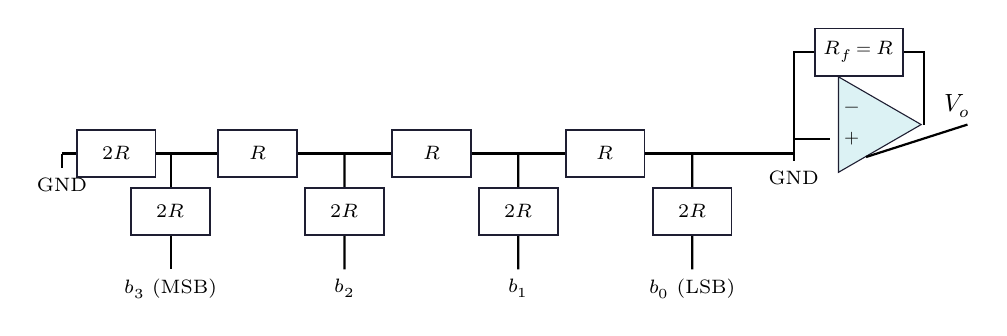
\begin{tikzpicture}[scale=0.92]
  % Nodes
  \coordinate (n3) at (0, 0);
  \coordinate (n2) at (2.4, 0);
  \coordinate (n1) at (4.8, 0);
  \coordinate (n0) at (7.2, 0);

  % Horizontal Resistors R
  \draw[thick] (-1.5, 0) -- (n3);
  \node[resnode] at (-0.75, 0) {$2R$};
  \node[below, font=\scriptsize] at (-1.5, -0.2) {GND};
  \draw[thick] (-1.5, 0) -- (-1.5, -0.2);

  \draw[thick] (n3) -- (n2);
  \node[resnode] at (1.2, 0) {$R$};

  \draw[thick] (n2) -- (n1);
  \node[resnode] at (3.6, 0) {$R$};

  \draw[thick] (n1) -- (n0);
  \node[resnode] at (6.0, 0) {$R$};

  % Vertical Resistors 2R
  \draw[thick] (n3) -- (0, -1.6);
  \node[resnode] at (0, -0.8) {$2R$};
  \node[below, font=\scriptsize] at (0, -1.6) {$b_3$ (MSB)};

  \draw[thick] (n2) -- (2.4, -1.6);
  \node[resnode] at (2.4, -0.8) {$2R$};
  \node[below, font=\scriptsize] at (2.4, -1.6) {$b_2$};

  \draw[thick] (n1) -- (4.8, -1.6);
  \node[resnode] at (4.8, -0.8) {$2R$};
  \node[below, font=\scriptsize] at (4.8, -1.6) {$b_1$};

  \draw[thick] (n0) -- (7.2, -1.6);
  \node[resnode] at (7.2, -0.8) {$2R$};
  \node[below, font=\scriptsize] at (7.2, -1.6) {$b_0$ (LSB)};

  % Op-amp Summing stage
  \draw[thick] (n0) -- (8.6, 0) -- (8.6, 0.6);
  \node[draw=mydark, fill=hdrteal, regular polygon, regular polygon sides=3, rotate=-90, minimum size=1.4cm] (opamp) at (9.6, 0.4) {};
  \node[font=\scriptsize] at (9.4, 0.6) {$-$};
  \node[font=\scriptsize] at (9.4, 0.2) {$+$};
  \draw[thick] (9.1, 0.2) -- (8.6, 0.2) -- (8.6, -0.1);
  \node[below, font=\scriptsize] at (8.6, -0.1) {GND};

  \draw[thick] (opamp.east) -- (11.0, 0.4) node[pos=0.9, above, font=\small] {$V_o$};
  \draw[thick] (8.6, 0.6) -- (8.6, 1.4) -- (10.4, 1.4) -- (10.4, 0.4);
  \node[resnode] at (9.5, 1.4) {$R_f = R$};
\end{tikzpicture}
\end{tcolorbox}

For an $n$-bit $R\text{-}2R$ ladder DAC, the analog output voltage is:
\begin{equation}
  V_o = -V_{\text{ref}} \frac{R_f}{R} \sum_{i=1}^{n} \frac{b_i}{2^i} = -V_{\text{ref}} \left( \frac{b_1}{2} + \frac{b_2}{4} + \dots + \frac{b_n}{2^n} \right) \quad (\text{when } R_f = R)
\end{equation}
\textbf{Key Advantages:}
\begin{itemize}[leftmargin=*, itemsep=2pt]
  \item Requires only two values: $R$ and $2R$.
  \item Highly practical for monolithic semiconductor IC fabrication using thin-film laser-trimmed resistors.
  \item Easily scalable to high bit-resolutions ($12$, $16$, or $24$ bits).
\end{itemize}

% ===============================================================================
\section{Analog-to-Digital Converters (ADC)}
% ===============================================================================

An ADC converts a continuous-time, continuous-amplitude analog voltage $V_{in}$ into a discrete $n$-bit digital code via three sequential steps: \textbf{Sampling, Quantization, and Binary Encoding}.

\subsection{Quantization Error and ADC Dynamic Range}
The ideal quantization step size is $\Delta = \frac{V_{FS}}{2^n - 1}$. The maximum inherent quantization uncertainty is:
\begin{equation}
  Q_e = \pm \frac{\Delta}{2}
\end{equation}
The theoretical Signal-to-Quantization-Noise Ratio (SQNR) for a full-scale sinusoidal input is:
\begin{equation}
  \text{SQNR} = 6.02 n + 1.76 \text{ dB}
\end{equation}
Every added bit of resolution improves dynamic range by approximately $6\text{ dB}$.

\subsection{Flash (Simultaneous / Parallel) ADC}
The Flash ADC is the \textbf{fastest possible ADC architecture}.
\begin{itemize}[leftmargin=*, itemsep=3pt]
  \item \textbf{Architecture:} Contains a precision reference voltage divider of $2^n$ identical resistors generating $2^n - 1$ reference thresholds, $2^n - 1$ analog comparators operating in parallel, and a priority encoder.
  \item \textbf{Operation:} All $2^n - 1$ comparators simultaneously compare $V_{in}$ against their assigned reference levels in a single clock cycle, generating a thermometer code which is converted to binary by the priority encoder.
  \item \textbf{Conversion Time:} Strictly $1$ clock cycle ($O(1)$ time complexity, typically $< 1\text{--}5\text{ ns}$).
  \item \textbf{Limitation:} Circuit hardware grows exponentially ($2^n - 1$ comparators). An 8-bit Flash ADC requires $255$ comparators; a 10-bit converter requires $1{,}023$ comparators, resulting in huge silicon area and excessive power consumption.
\end{itemize}

\subsection{Successive Approximation Register (SAR) ADC}
The SAR ADC utilizes a \textbf{binary search algorithm} to systematically approximate the input voltage bit by bit from MSB down to LSB using a single comparator and an internal DAC.
\begin{enumerate}[label=\arabic*., leftmargin=*]
  \item \textbf{Cycle 1:} The SAR sets the MSB ($b_1 = 1$, all others $0$). The DAC generates $V_{\text{DAC}} = \frac{1}{2} V_{\text{ref}}$.
  \item If $V_{in} > V_{\text{DAC}}$, the comparator output is HIGH; the MSB is retained ($b_1 = 1$). If $V_{in} < V_{\text{DAC}}$, the MSB is cleared ($b_1 = 0$).
  \item \textbf{Cycle 2 to $n$:} The process is repeated sequentially for each successive bit ($b_2, b_3, \dots, b_n$).
  \item \textbf{Conversion Time:} Strictly constant and directly proportional to resolution:
  \begin{equation}
    T_C = n \times T_{\text{clk}}
  \end{equation}
  \item \textbf{Applications:} The industry standard for medium-to-high speed ($100\text{ kSPS}$ to $10\text{ MSPS}$), $10\text{--}18\text{ bit}$ instrumentation, biomedical data acquisition (ECG/EEG), and microcontroller embedded ADCs.
\end{enumerate}

\subsection{Dual-Slope Integrating ADC}
The Dual-Slope ADC provides the \textbf{highest accuracy and superior noise rejection} through continuous analog integration.

\begin{tcolorbox}[defbox, title={\textbf{Dual-Slope Conversion Derivation}}]
\begin{itemize}[leftmargin=*, itemsep=3pt]
  \item \textbf{Phase 1 (Fixed-Time Run-Up):} Switch connects to $V_{in}$ for a fixed time $T_1 = 2^n \times T_{\text{clk}}$. The integrator output ramps to a peak voltage:
  \begin{equation}
    V_{\text{peak}} = -\frac{1}{RC} \int_{0}^{T_1} V_{in} \, dt = -\frac{V_{in} T_1}{RC}
  \end{equation}
  \item \textbf{Phase 2 (Variable-Time Run-Down):} Switch connects to a negative reference $-V_{\text{ref}}$. The integrator ramps back toward zero at a constant slope:
  \begin{equation}
    V_o(t) = V_{\text{peak}} + \frac{V_{\text{ref}} t}{RC}
  \end{equation}
  When $V_o(t) = 0$ at time $t = T_2$, the comparator stops the digital counter.
  \item Equating integrator charges:
  \begin{equation}
    \frac{V_{in} T_1}{RC} = \frac{V_{\text{ref}} T_2}{RC} \implies T_2 = T_1 \left(\frac{V_{in}}{V_{\text{ref}}}\right)
  \end{equation}
\end{itemize}
\end{tcolorbox}

\textbf{Outstanding Advantages:}
\begin{itemize}[leftmargin=*, itemsep=2pt]
  \item \textbf{Immune to Component Drift:} Conversion time $T_2$ is \textbf{entirely independent of the integration resistance $R$, capacitance $C$, and clock frequency $f_{\text{clk}}$} because they cancel out completely in the ratio.
  \item \textbf{Power-Line Noise Rejection:} By setting integration period $T_1$ to an exact integer multiple of the $50\text{ Hz}$ or $60\text{ Hz}$ power-line cycle ($20\text{ ms}$ or $16.67\text{ ms}$), hum and line noise integrate to identically zero.
  \item \textbf{Limitation:} Very slow conversion ($T_{C(\max)} = 2 \times 2^n \times T_{\text{clk}}$). Standard choice for precision Digital Multimeters (DMMs) and digital weigh scales.
\end{itemize}

\par\vspace{6pt}\noindent
\begingroup
\setlength{\tabcolsep}{3.5pt}
\setlength{\extrarowheight}{3pt}
\begin{tabularx}{\linewidth}{|B{2.2cm}|Y|Y|Y|Y|}
\hline
\textbf{Parameter} & \textbf{Flash ADC} & \textbf{SAR ADC} & \textbf{Dual-Slope ADC} & \textbf{Counter / Ramp ADC} \\
\hline
Conversion Speed & Extremely Fast ($1\text{--}5\text{ ns}$) & Fast ($1\text{--}10\,\mu\text{s}$) & Extremely Slow ($10\text{--}100\text{ ms}$) & Slow (Variable) \\
\hline
Clock Cycles & $1$ clock cycle ($O(1)$) & $n$ clock cycles & Up to $2 \times 2^n$ cycles & Up to $2^n$ cycles \\
\hline
Resolution & $6\text{--}8$ bits & $8\text{--}18$ bits & $16\text{--}24$ bits (Highest) & $8\text{--}10$ bits \\
\hline
\end{tabularx}
\endgroup

\par\vspace{6pt}\noindent
\begingroup
\setlength{\tabcolsep}{3.5pt}
\setlength{\extrarowheight}{3pt}
\begin{tabularx}{\linewidth}{|B{2.2cm}|Y|Y|Y|Y|}
\hline
\textbf{Parameter (contd.)} & \textbf{Flash ADC} & \textbf{SAR ADC} & \textbf{Dual-Slope ADC} & \textbf{Counter / Ramp ADC} \\
\hline
Hardware Cost & High ($2^n - 1$ comparators) & Moderate ($1$ comp, $1$ DAC) & Low ($1$ integrator, $1$ comp) & Low ($1$ counter, $1$ DAC) \\
\hline
Noise Immunity & Poor & Moderate & Exceptional ($50/60\text{ Hz}$ hum) & Poor \\
\hline
Typical Uses & Radar, oscilloscopes, video & Microcontrollers, DSP & DMMs, weighing scales & Low-cost sensors \\
\hline
\end{tabularx}
\endgroup

% ===============================================================================
\section{Sample and Hold (S/H) Circuit}
% ===============================================================================

When converting high-frequency analog signals, any input variation during the finite conversion interval ($t_c$) introduces \textbf{aperture error}. A Sample-and-Hold circuit freezes the analog voltage for the duration of the ADC conversion.

\subsection{Circuit Topology and Modes of Operation}
A basic S/H circuit consists of an input unity-gain buffer op-amp, a high-speed analog switch (JFET or MOSFET), an ultra-low leakage \textbf{Hold Capacitor ($C_H$)}, and an output high-input-impedance unity-gain buffer op-amp.
\begin{itemize}[leftmargin=*, itemsep=3pt]
  \item \textbf{Sample (Track) Mode:} The switch is closed (ON). The hold capacitor $C_H$ charges to follow the input analog voltage $V_{in}$ through the switch ON resistance $R_{\text{on}}$.
  \item \textbf{Hold Mode:} The switch is opened (OFF). The charge trapped on $C_H$ maintains the instantaneous voltage constant. The high-impedance buffer delivers this stable voltage to the ADC.
\end{itemize}

\subsection{Key Dynamic Performance Parameters}
\begin{itemize}[leftmargin=*, itemsep=3pt]
  \item \textbf{Acquisition Time ($t_{ac}$):} Time required for the hold capacitor voltage to charge and settle to within a specified error band (e.g., $0.01\%$ or $\pm \frac{1}{2}\text{ LSB}$) following a transition from hold to sample mode. Governed by switch resistance and capacitance:
  \begin{equation}
    t_{ac} \approx k \cdot R_{\text{on}} \cdot C_H \quad (\text{where } k \approx 7\text{--}9 \text{ for 12-bit accuracy})
  \end{equation}
  \item \textbf{Aperture Time ($t_{ap}$):} The finite delay between the initiation of the hold command and the effective physical opening of the sampling switch.
  \item \textbf{Aperture Jitter ($t_j$):} The sample-to-sample statistical timing uncertainty in switch opening. The maximum input signal frequency before aperture jitter exceeds $1\text{ LSB}$ is:
  \begin{equation}
    f_{\max} = \frac{1}{2\pi \cdot t_j \cdot 2^n}
  \end{equation}
  \item \textbf{Droop Rate ($\frac{dV}{dt}$):} The rate at which the output voltage drifts during hold mode due to capacitor discharge through parasitic leakage currents:
  \begin{equation}
    \text{Droop Rate} = \frac{I_{\text{leak}}}{C_H}
  \end{equation}
  \item \textbf{Trade-off in Sizing $C_H$:} A large $C_H$ reduces droop rate but increases acquisition time; a small $C_H$ accelerates acquisition but degrades droop performance.
\end{itemize}

\newpage
% ===============================================================================
\section{Quick Revision Page}
% ===============================================================================

\begin{tcolorbox}[formulabox, title={\textbf{Key Formulas and Characteristic Relations at a Glance}}]
\begin{itemize}[leftmargin=*, itemsep=3pt]
  \item \textbf{Digital IC Speed-Power Metric:}
  \begin{equation*}
    t_{pd} = \frac{t_{PLH} + t_{PHL}}{2}, \quad \text{PDP} = P_D \times t_{pd}, \quad P_{\text{dyn(CMOS)}} = \alpha C_L V_{DD}^2 f
  \end{equation*}
  \item \textbf{Noise Margins and Open-Collector Pull-up Resistor:}
  \begin{equation*}
    NM_H = V_{OH(\min)} - V_{IH(\min)}, \quad NM_L = V_{IL(\max)} - V_{OL(\max)}, \quad R_{P(\min)} = \frac{V_{CC} - V_{OL}}{I_{OL} - N \cdot I_{IL}}
  \end{equation*}
  \item \textbf{DAC Resolution and Analog Output ($R\text{-}2R$ Ladder):}
  \begin{equation*}
    \text{Step Size} = \frac{V_{FS}}{2^n - 1}, \quad V_o = -V_{\text{ref}} \left(\frac{b_1}{2} + \frac{b_2}{4} + \dots + \frac{b_n}{2^n}\right)
  \end{equation*}
  \item \textbf{ADC Timing and Dual-Slope Relation:}
  \begin{equation*}
    T_{C(\text{SAR})} = n \cdot T_{\text{clk}}, \quad T_{C(\text{Flash})} = 1 \cdot T_{\text{clk}}, \quad T_2 = T_1 \cdot \left(\frac{V_{in}}{V_{\text{ref}}}\right)
  \end{equation*}
\end{itemize}
\end{tcolorbox}

\begin{tcolorbox}[defbox, title={\textbf{One-Line High-Yield Definitions}}]
\begin{itemize}[leftmargin=*, itemsep=2pt]
  \item \textbf{Noise Margin:} The maximum noise voltage amplitude that can be added to an input signal without corrupting the recognized logic level.
  \item \textbf{Totem-Pole Output:} An active BJT push-pull output driver providing low impedance during both pull-up and pull-down transitions.
  \item \textbf{ECL Logic Family:} Non-saturating BJT current-steering logic that avoids saturation charge storage to achieve sub-nanosecond speeds.
  \item \textbf{Static RAM (SRAM):} Volatile memory storing data in bi-stable cross-coupled CMOS inverters requiring no periodic refresh.
  \item \textbf{Dynamic RAM (DRAM):} Volatile memory storing data as charge on a 1T-1C capacitor requiring periodic refresh cycles.
  \item \textbf{Look-Up Table (LUT):} An SRAM-based truth table in an FPGA that realizes any arbitrary $k$-variable logic function.
  \item \textbf{Flash ADC:} A parallel ADC utilizing $2^n - 1$ simultaneous comparators to perform conversions in a single clock cycle.
  \item \textbf{Dual-Slope ADC:} An integrating ADC whose conversion is independent of $R$, $C$, and clock frequency, offering high noise rejection.
  \item \textbf{SAR ADC:} An analog-to-digital converter that determines binary bits sequentially via a binary search algorithm in $n$ cycles.
  \item \textbf{Droop Rate:} The rate of voltage decay across the hold capacitor in a Sample-and-Hold circuit caused by parasitic leakage.
\end{itemize}
\end{tcolorbox}

\begin{tcolorbox}[exambox, title={\textbf{Frequently Asked / Viva Questions}}]
\begin{enumerate}[label=\arabic*., leftmargin=*]
  \item \Q{Why can totem-pole TTL outputs not be connected in a wired-AND configuration?}
  If one gate asserts HIGH and the other LOW, a direct low-resistance short circuit from $V_{CC}$ to ground through $Q_3$ and $Q_4$ occurs, producing damaging current spikes and destruction.

  \item \Q{Why is ECL significantly faster than TTL?}
  ECL operates BJTs strictly in the non-saturating active region using a differential current-steering switch. Eliminating saturation eliminates base minority carrier storage time ($t_s = 0$).

  \item \Q{Why does static CMOS consume virtually zero power at DC?}
  For any stable logic input, either the PMOS pull-up network or the NMOS pull-down network is completely turned OFF, cutting off any direct path between $V_{DD}$ and ground.

  \item \Q{Why must PMOS transistors be made wider than NMOS in CMOS inverters?}
  Because electron mobility in silicon is approximately $2.5$ times higher than hole mobility ($\mu_n \approx 2.5 \mu_p$). PMOS width must be scaled by $2.5\times$ to equalize drive currents.

  \item \Q{Why does DRAM require periodic refreshing while SRAM does not?}
  DRAM stores data as charge on tiny capacitors ($C_s \approx 30\text{ fF}$) which leak through semiconductor junctions within milliseconds. SRAM uses cross-coupled active latching inverters.

  \item \Q{Explain the functional architectural difference between PLA and PAL.}
  A PLA features both programmable AND and programmable OR arrays, offering maximum term sharing. A PAL has a programmable AND array and a fixed OR array, offering faster speed and simpler structure.

  \item \Q{What is a Look-Up Table (LUT) in an FPGA?}
  An LUT is a small SRAM block storing the truth table values of a logic function. For a 4-input LUT, 4 input lines act as addresses selecting 1 of 16 stored output bits.

  \item \Q{Why is an $R\text{-}2R$ ladder DAC preferred over a binary-weighted resistor DAC?}
  An $R\text{-}2R$ ladder requires only two resistor values ($R$ and $2R$) regardless of bit resolution, avoiding the fabrication of massive, tightly matched resistor ranges.

  \item \Q{How many comparators are required for an 8-bit Flash ADC?}
  An 8-bit Flash ADC requires $2^8 - 1 = 255$ parallel comparators.

  \item \Q{Why is conversion time constant in a SAR ADC regardless of input voltage?}
  Because a SAR ADC always executes a fixed $n$-step binary search sequence, testing one bit per clock cycle from MSB to LSB.

  \item \Q{Why is the Dual-Slope ADC immune to variations in resistance and capacitance?}
  Because the integrator component values $R$ and $C$ appear identically in both the run-up and run-down equations and cancel out completely in the ratio $T_2 = T_1 (V_{in}/V_{\text{ref}})$.

  \item \Q{What causes aperture jitter in a Sample-and-Hold circuit, and why is it problematic?}
  Aperture jitter is the sample-to-sample statistical variation in the switch opening moment, which introduces phase noise and voltage errors when sampling fast-changing analog signals.
\end{enumerate}
\end{tcolorbox}

\begin{tcolorbox}[tikzbox, title={\textbf{Summary Matrix: Comparison of ADC Architectures}}]
\centering
\begingroup
\setlength{\tabcolsep}{4pt}
\setlength{\extrarowheight}{3pt}
\begin{tabularx}{\linewidth}{|B{3.2cm}|Y|Y|Y|}
\hline
\textbf{Metric} & \textbf{Flash ADC} & \textbf{SAR ADC} & \textbf{Dual-Slope ADC} \\
\hline
Conversion Time ($T_C$) & $1$ clock cycle ($O(1)$) & $n$ clock cycles ($O(n)$) & Up to $2^{n+1}$ cycles ($O(2^n)$) \\
\hline
Relative Speed & Ultra-fast ($> 1\text{ GSPS}$) & Medium-high ($100\text{ kSPS}$--$10\text{ MSPS}$) & Very slow ($10$--$100\text{ SPS}$) \\
\hline
Hardware Complexity & Exponential ($2^n - 1$ comparators) & Moderate ($1$ comp, $1$ DAC, SAR) & Minimal ($1$ integrator, $1$ comp) \\
\hline
Resolution Limits & $6\text{--}8$ bits (rarely 10) & $8\text{--}18$ bits & $16\text{--}24$ bits (Extreme precision) \\
\hline
Noise Rejection & Poor & Moderate & Superb (line hum canceling) \\
\hline
Dominant Usage & Oscilloscopes, SDR, radar & Embedded MCUs, audio, DSP & Digital multimeters, scales \\
\hline
\end{tabularx}
\endgroup
\end{tcolorbox}


% -- Module 4 -----------------------------------------------------------------
\modulestart{4}{The VLSI Design Flow and Methodologies}

\section{The VLSI Design Flow and Methodologies}
% ===============================================================================

Very Large Scale Integration (VLSI) design is the systematic transformation of an abstract architectural system specification into a physically verified, fabricated silicon integrated circuit containing millions to billions of transistors.

\subsection{The Gajski-Kuhn Y-Chart}
The Gajski-Kuhn Y-chart visualizes VLSI design complexity across three distinct \textbf{domains of representation} intersecting at concentric \textbf{levels of abstraction}:
\begin{itemize}[leftmargin=*, itemsep=3pt]
  \item \textbf{Behavioral Domain (What it does):} Specifies functional algorithms, equations, input-output relationships, and state transitions without detailing physical hardware.
  \item \textbf{Structural Domain (How it is composed):} Defines hardware entities as interconnections of structural sub-blocks, modules, logic gates, and transistors.
  \item \textbf{Physical / Geometric Domain (How it is built):} Represents physical implementation as silicon geometric masks, transistor layouts, placement coordinates, and metallization routing tracks.
  \item \textbf{Levels of Abstraction:} Architectural / System level $\to$ Algorithmic level $\to$ Register-Transfer Level (RTL) $\to$ Logic / Gate level $\to$ Transistor / Circuit level $\to$ Mask layout level.
\end{itemize}

\subsection{Step-by-Step Modern Digital ASIC and FPGA Design Flow}
\begin{enumerate}[label=\arabic*., leftmargin=*]
  \item \textbf{System Specification \& Architecture Planning:} Defines system throughput, clock frequency, word width, power budget, and interface protocols.
  \item \textbf{Design Entry:} Entering the digital design into CAD tools:
    \begin{itemize}
      \item \textit{Schematic Capture:} Graphical drawing of interconnected logic gates. Intuitive for small designs; unmanageable for complex million-gate chips.
      \item \textit{State Diagram / FSM Entry:} Graphical specification of states, transitions, and outputs; automatically compiled into HDL code.
      \item \textit{Hardware Description Languages (HDLs):} Textual algorithmic descriptions using VHDL, Verilog, or SystemVerilog. Standard for modern complex VLSI.
    \end{itemize}
  \item \textbf{Functional (RTL) Simulation:} Verifies behavioral and logic correctness using an HDL testbench. Assumes ideal zero-delay or unit-delay gates to detect algorithmic bugs early.
  \item \textbf{Logic Synthesis:} CAD tool (e.g., Synopsys Design Compiler, Vivado) translates abstract RTL code into an optimized, technology-specific \textbf{gate-level netlist} mapped to standard cells (AND, NAND, Flip-Flops) from a target semiconductor library, driven by designer constraints (target clock period, maximum silicon area, dynamic power).
  \item \textbf{Gate-Level Netlist Simulation:} Simulates the synthesized gate netlist to confirm that synthesis introduced no unintended logic changes or state mismatches.
  \item \textbf{Static Timing Analysis (STA):} Exhaustively evaluates path delays to guarantee that clock setup and hold time requirements are met for every register without dynamic vectors:
    \begin{align}
      \text{Setup Time Constraint:} \quad & T_{\text{clk}} \ge t_{cq} + t_{\text{comb}(\max)} + t_{\text{setup}} - t_{\text{skew}} \\
      \text{Hold Time Constraint:} \quad & t_{cq} + t_{\text{comb}(\min)} \ge t_{\text{hold}} + t_{\text{skew}}
    \end{align}
  \item \textbf{Physical Design (P\&R - Place and Route):}
    \begin{itemize}
      \item \textit{Floorplanning:} Allocates chip area for major functional blocks, I/O pads, and power/ground grids ($V_{DD}, V_{SS}$).
      \item \textit{Placement:} Determines exact $(x, y)$ coordinate locations for every standard cell.
      \item \textit{Clock Tree Synthesis (CTS):} Constructs balanced clock distribution networks (H-tree) to minimize clock skew ($t_{\text{skew}}$) and insertion delay.
      \item \textit{Routing:} Wires together all cell pins using multi-layer metallization.
    \end{itemize}
  \item \textbf{Parasitic Extraction and Post-Layout Timing Verification:} Extracts parasitic resistances ($R$) and capacitances ($C$) from actual layout geometries and back-annotates them into a Standard Delay Format (SDF) file for final timing sign-off.
  \item \textbf{Physical Verification:}
    \begin{itemize}
      \item \textit{DRC (Design Rule Checking):} Verifies that geometric shapes satisfy foundry manufacturing rules (minimum metal width, spacing, enclosure).
      \item \textit{LVS (Layout Versus Schematic):} Extracts electrical transistor circuits from the physical layout and compares connectivity netlists 1-to-1 against the schematic.
    \end{itemize}
  \item \textbf{Tape-out:} Exporting final layout data in GDSII / OASIS stream format to the semiconductor foundry for photolithographic mask fabrication (or generating a configuration bitstream for an FPGA).
\end{enumerate}

\begin{tcolorbox}[tikzbox, title={Digital VLSI / ASIC Design Flow Pipeline}]
\centering
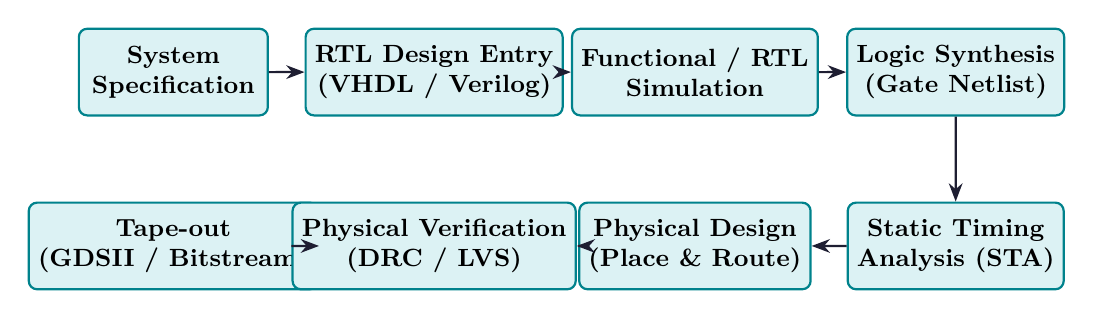
\begin{tikzpicture}[scale=0.92]
  \node[vlsiblock] (s1) at (0, 3.6) {System\\Specification};
  \node[vlsiblock] (s2) at (3.6, 3.6) {RTL Design Entry\\(VHDL / Verilog)};
  \node[vlsiblock] (s3) at (7.2, 3.6) {Functional / RTL\\Simulation};
  \node[vlsiblock] (s4) at (10.8, 3.6) {Logic Synthesis\\(Gate Netlist)};

  \node[vlsiblock] (s8) at (0, 1.2) {Tape-out\\(GDSII / Bitstream)};
  \node[vlsiblock] (s7) at (3.6, 1.2) {Physical Verification\\(DRC / LVS)};
  \node[vlsiblock] (s6) at (7.2, 1.2) {Physical Design\\(Place \& Route)};
  \node[vlsiblock] (s5) at (10.8, 1.2) {Static Timing\\Analysis (STA)};

  \draw[flowarrow] (s1) -- (s2);
  \draw[flowarrow] (s2) -- (s3);
  \draw[flowarrow] (s3) -- (s4);
  \draw[flowarrow] (s4) -- (s5);
  \draw[flowarrow] (s5) -- (s6);
  \draw[flowarrow] (s6) -- (s7);
  \draw[flowarrow] (s7) -- (s8);
\end{tikzpicture}
\end{tcolorbox}

% ===============================================================================
\section{VHDL Language Fundamentals and Structural Units}
% ===============================================================================

VHDL (VHSIC Hardware Description Language) is an IEEE standard (IEEE Std 1076) language designed to model the behavior, dataflow, and structural composition of digital electronic systems across multiple levels of abstraction.

\subsection{Fundamental Design Units of VHDL}
A complete VHDL design entity is composed of primary design units:
\begin{enumerate}[label=\arabic*., leftmargin=*]
  \item \textbf{Library and Package Declarations:} Grants access to pre-compiled packages containing standardized data types, constants, and operators:
\begin{spacing}{1.0}
\begin{verbatim}
LIBRARY IEEE;
USE IEEE.STD_LOGIC_1164.ALL;    -- Imports STD_LOGIC, STD_LOGIC_VECTOR
USE IEEE.NUMERIC_STD.ALL;       -- Imports SIGNED, UNSIGNED arithmetic
\end{verbatim}
\end{spacing}
  \item \textbf{Entity Declaration:} Defines the external hardware boundary and interface ports of the module (the "black box" view):
\begin{spacing}{1.0}
\begin{verbatim}
ENTITY entity_name IS
  GENERIC ( param_name : type := default_val ); -- Optional parameterized constants
  PORT (
    port_name : mode data_type;
    ...
  );
END entity_name;
\end{verbatim}
\end{spacing}
  \item \textbf{Architecture Body:} Defines the internal behavior, logic equations, or structural interconnection of components (the "inside" of the box). Multiple architectures can be written for a single entity (e.g., behavioral vs. structural):
\begin{spacing}{1.0}
\begin{verbatim}
ARCHITECTURE arch_name OF entity_name IS
  -- Declarative region: signals, constants, components, types
BEGIN
  -- Concurrent statements region: processes, component instantiations
END arch_name;
\end{verbatim}
\end{spacing}
  \item \textbf{Configuration Declaration:} Binds specific architecture bodies and component implementations to entity instances in hierarchical designs.
\end{enumerate}

\subsection{VHDL Port Modes}
\par\vspace{6pt}\noindent
\begingroup
\setlength{\tabcolsep}{3.5pt}
\setlength{\extrarowheight}{3pt}
\begin{tabularx}{\linewidth}{|B{2.2cm}|B{3.2cm}|Y|}
\hline
\textbf{Port Mode} & \textbf{Directionality} & \textbf{Internal Architecture Usage} \\
\hline
\texttt{IN} & Input to module & Read-only inside architecture. Cannot be assigned or driven. \\
\hline
\texttt{OUT} & Output from module & Write-only. Values can be assigned to it, but cannot be read internally. \\
\hline
\texttt{INOUT} & Bidirectional & Can be driven and read internally. Requires tri-state resolution. \\
\hline
\texttt{BUFFER} & Output with internal feedback & Drives output pin and allows internal readback. Has restrictive binding rules. \\
\hline
\end{tabularx}
\endgroup

% ===============================================================================
\section{Data Types, Data Objects, and Operators}
% ===============================================================================

\subsection{Data Objects in VHDL}
VHDL supports four classes of data objects:
\begin{itemize}[leftmargin=*, itemsep=4pt]
  \item \textbf{SIGNAL:} Represents physical interconnecting electrical wires or traces.
    \begin{itemize}
      \item Declared in architecture declarative regions or packages; visible throughout the entire architecture.
      \item Updated concurrently with a scheduled propagation delay (delta delay $\delta$).
      \item Assignment operator: \texttt{<=} (e.g., \texttt{Y <= A AND B;}).
    \end{itemize}
  \item \textbf{VARIABLE:} Represents local computational scratchpad storage.
    \begin{itemize}
      \item Declared strictly inside a \texttt{PROCESS}, \texttt{FUNCTION}, or \texttt{PROCEDURE}. Not visible outside.
      \item Updated \textbf{instantaneously} without delay.
      \item Assignment operator: \texttt{:=} (e.g., \texttt{v\_count := v\_count + 1;}).
    \end{itemize}
  \item \textbf{CONSTANT:} Holds a permanent, unmodifiable value established during elaboration. Assignment operator: \texttt{:=} (e.g., \texttt{CONSTANT WIDTH : INTEGER := 8;}).
  \item \textbf{FILE:} Represents external host system files used for automated testbench verification and stimulus vectors.
\end{itemize}

\par\vspace{6pt}\noindent
\begingroup
\setlength{\tabcolsep}{3.5pt}
\setlength{\extrarowheight}{3pt}
\begin{tabularx}{\linewidth}{|B{2.8cm}|Y|Y|}
\hline
\textbf{Property} & \textbf{SIGNAL} & \textbf{VARIABLE} \\
\hline
Hardware Meaning & Physical electrical wire / bus & Local memory / register variable \\
\hline
Declaration Scope & Architecture, package, block & Exclusively inside \texttt{PROCESS} or subprograms \\
\hline
Assignment Operator & \texttt{<=} (Non-blocking, scheduled) & \texttt{:=} (Blocking, instantaneous) \\
\hline
Update Timing & Updated at end of current simulation cycle & Updated immediately when evaluated \\
\hline
Synthesized Hardware & Interconnecting wires, latches, or flip-flops & Internal combinational nodes or registers \\
\hline
\end{tabularx}
\endgroup

\subsection{Standard and IEEE 1164 Data Types}
\begin{itemize}[leftmargin=*, itemsep=3pt]
  \item \textbf{Standard Types:} \texttt{BIT} (\texttt{'0'}, \texttt{'1'}), \texttt{BOOLEAN} (\texttt{TRUE}, \texttt{FALSE}), \texttt{INTEGER} (32-bit minimum range: $-2^{31}$ to $2^{31}-1$), \texttt{CHARACTER}, \texttt{TIME} (e.g., \texttt{10 ns}).
  \item \textbf{IEEE Standard 1164 Multi-Valued Logic (\texttt{STD\_LOGIC}):} Provides realistic modeling of electrical logic states across integrated circuit nodes:
\end{itemize}

\par\vspace{6pt}\noindent
\begingroup
\setlength{\tabcolsep}{3.5pt}
\setlength{\extrarowheight}{3pt}
\begin{tabularx}{\linewidth}{|B{1.6cm}|B{3.2cm}|Y|}
\hline
\textbf{Value} & \textbf{Electrical Meaning} & \textbf{Hardware Significance} \\
\hline
\texttt{'U'} & Uninitialized & Default initial simulation state of unassigned signals \\
\hline
\texttt{'X'} & Forcing Unknown & Unresolvable contention / unknown logic conflict \\
\hline
\texttt{'0'} & Forcing 0 & Strong logic LOW tied to ground ($V_{SS}$) \\
\hline
\texttt{'1'} & Forcing 1 & Strong logic HIGH tied to supply ($V_{DD}$) \\
\hline
\texttt{'Z'} & High Impedance & Tri-state output; electrically disconnected \\
\hline
\texttt{'W'} & Weak Unknown & Weak signal contention \\
\hline
\texttt{'L'} & Weak 0 & Pull-down resistor to ground \\
\hline
\texttt{'H'} & Weak 1 & Pull-up resistor to supply \\
\hline
\texttt{'-'} & Don't Care & Wildcard used in synthesis minimization \\
\hline
\end{tabularx}
\endgroup

\subsection{VHDL Operators}
\begin{itemize}[leftmargin=*, itemsep=2pt]
  \item \textbf{Logical Operators:} \texttt{AND}, \texttt{OR}, \texttt{NAND}, \texttt{NOR}, \texttt{XOR}, \texttt{XNOR}, \texttt{NOT}.
  \item \textbf{Relational Operators:} \texttt{=} (equal), \texttt{/=} (not equal), \texttt{<}, \texttt{<=}, \texttt{>}, \texttt{>=}.
  \item \textbf{Arithmetic Operators:} \texttt{+} (addition), \texttt{-} (subtraction), \texttt{*} (multiplication), \texttt{/} (division), \texttt{MOD}, \texttt{REM}, \texttt{ABS}, \texttt{**} (exponentiation).
  \item \textbf{Concatenation Operator (\texttt{\&}):} Combines scalars or vectors into wider vectors (e.g., \texttt{Y <= A \& B;}).
\end{itemize}

% ===============================================================================
\section{VHDL Modeling Styles and Coding Methodologies}
% ===============================================================================

Digital hardware architectures can be expressed using three distinct modeling styles:

\subsection{Dataflow (Concurrent) Modeling}
Expresses hardware as continuous concurrent signal assignments that execute simultaneously whenever any right-hand-side operand changes:
\begin{itemize}[leftmargin=*, itemsep=3pt]
  \item \textbf{Simple Concurrent Assignment:} \texttt{Y <= A AND B;}
  \item \textbf{Conditional Signal Assignment (\texttt{WHEN-ELSE}):}
\begin{spacing}{1.0}
\begin{verbatim}
Y <= A WHEN (Sel = "00") ELSE
     B WHEN (Sel = "01") ELSE
     C WHEN (Sel = "10") ELSE D;
\end{verbatim}
\end{spacing}
  \item \textbf{Selected Signal Assignment (\texttt{WITH-SELECT}):}
\begin{spacing}{1.0}
\begin{verbatim}
WITH Sel SELECT
  Y <= A WHEN "00",
       B WHEN "01",
       C WHEN "10",
       D WHEN OTHERS;
\end{verbatim}
\end{spacing}
\end{itemize}

\subsection{Behavioral (Sequential) Modeling}
Specifies the algorithmic behavior of the hardware within a \textbf{\texttt{PROCESS}} block. Statements inside a process execute sequentially from top to bottom, but the process block itself is evaluated concurrently relative to the rest of the architecture:
\begin{itemize}[leftmargin=*, itemsep=3pt]
  \item \textbf{Sensitivity List:} A list of signals enclosed in parentheses following the \texttt{PROCESS} keyword. The process activates whenever any signal in its sensitivity list transitions:
\begin{spacing}{1.0}
\begin{verbatim}
PROCESS (clk, reset) -- Activated on transitions of clk or reset
BEGIN
  IF (reset = '1') THEN
    Q <= '0';
  ELSIF rising_edge(clk) THEN
    Q <= D;
  END IF;
END PROCESS;
\end{verbatim}
\end{spacing}
  \item \textbf{Sequential Control Statements:} \texttt{IF-THEN-ELSIF-ELSE}, \texttt{CASE-WHEN}, \texttt{FOR-LOOP}, \texttt{WHILE-LOOP}.
\end{itemize}

\begin{tcolorbox}[defbox, title={\textbf{Critical Synthesis Hazard: Inferred Latches}}]
In combinational processes, if an \texttt{IF} statement lacks a complete \texttt{ELSE} clause, or a \texttt{CASE} statement omits the \texttt{WHEN OTHERS} branch or fails to assign every output signal across all possible input permutations, the synthesis tool must infer a \textbf{transparent latch} to preserve the previous output state. This creates asynchronous hazards, degrades timing closure, and must be prevented by assigning unambiguous default values at the top of every combinational process.
\end{tcolorbox}

\subsection{Structural Modeling}
Describes a system hierarchically by declaring pre-designed sub-components and mapping their ports together like an electrical schematic:
\begin{enumerate}[label=\arabic*., leftmargin=*]
  \item Declare component interface in architecture declarative region.
  \item Instantiate components in architecture body and connect signals using \texttt{PORT MAP}.
\end{enumerate}

% ===============================================================================
\section{VHDL Code Library for Combinational Logic Circuits}
% ===============================================================================

\begin{tcolorbox}[examplebox, title={1. Half Adder and Full Adder (Dataflow, Behavioral, Structural)}]
\begin{spacing}{0.95}
\begin{verbatim}
-- Half Adder (Dataflow)
LIBRARY IEEE;
USE IEEE.STD_LOGIC_1164.ALL;
ENTITY half_adder IS
  PORT ( A, B : IN STD_LOGIC; Sum, Cout : OUT STD_LOGIC );
END half_adder;
ARCHITECTURE dataflow OF half_adder IS
BEGIN
  Sum  <= A XOR B;
  Cout <= A AND B;
END dataflow;

-- Full Adder (Structural using 2 Half Adders + OR Gate)
LIBRARY IEEE;
USE IEEE.STD_LOGIC_1164.ALL;
ENTITY full_adder IS
  PORT ( A, B, Cin : IN STD_LOGIC; Sum, Cout : OUT STD_LOGIC );
END full_adder;
ARCHITECTURE structural OF full_adder IS
  COMPONENT half_adder
    PORT ( A, B : IN STD_LOGIC; Sum, Cout : OUT STD_LOGIC );
  END COMPONENT;
  SIGNAL s1, c1, c2 : STD_LOGIC;
BEGIN
  HA1: half_adder PORT MAP ( A => A, B => B, Sum => s1, Cout => c1 );
  HA2: half_adder PORT MAP ( A => s1, B => Cin, Sum => Sum, Cout => c2 );
  Cout <= c1 OR c2;
END structural;
\end{verbatim}
\end{spacing}
\end{tcolorbox}

\begin{tcolorbox}[examplebox, title={2. 4-to-1 Multiplexer (Dataflow and Behavioral)}]
\begin{spacing}{0.95}
\begin{verbatim}
LIBRARY IEEE;
USE IEEE.STD_LOGIC_1164.ALL;

ENTITY mux4to1 IS
  PORT (
    D   : IN  STD_LOGIC_VECTOR(3 DOWNTO 0);
    Sel : IN  STD_LOGIC_VECTOR(1 DOWNTO 0);
    Y   : OUT STD_LOGIC
  );
END mux4to1;

ARCHITECTURE behavioral OF mux4to1 IS
BEGIN
  PROCESS (D, Sel)
  BEGIN
    CASE Sel IS
      WHEN "00" => Y <= D(0);
      WHEN "01" => Y <= D(1);
      WHEN "10" => Y <= D(2);
      WHEN "11" => Y <= D(3);
      WHEN OTHERS => Y <= '0';
    END CASE;
  END PROCESS;
END behavioral;
\end{verbatim}
\end{spacing}
\end{tcolorbox}

\begin{tcolorbox}[examplebox, title={3. 2-to-4 Binary Decoder with Active-Low Enable}]
\begin{spacing}{0.95}
\begin{verbatim}
LIBRARY IEEE;
USE IEEE.STD_LOGIC_1164.ALL;

ENTITY decoder2to4 IS
  PORT (
    A     : IN  STD_LOGIC_VECTOR(1 DOWNTO 0);
    En_n  : IN  STD_LOGIC;                     -- Active-low enable
    Y     : OUT STD_LOGIC_VECTOR(3 DOWNTO 0)   -- Active-high outputs
  );
END decoder2to4;

ARCHITECTURE dataflow OF decoder2to4 IS
BEGIN
  Y <= "0001" WHEN (En_n = '0' AND A = "00") ELSE
       "0010" WHEN (En_n = '0' AND A = "01") ELSE
       "0100" WHEN (En_n = '0' AND A = "10") ELSE
       "1000" WHEN (En_n = '0' AND A = "11") ELSE
       "0000";
END dataflow;
\end{verbatim}
\end{spacing}
\end{tcolorbox}

\begin{tcolorbox}[examplebox, title={4. 4-Bit Arithmetic Logic Unit (ALU)}]
\begin{spacing}{0.95}
\begin{verbatim}
LIBRARY IEEE;
USE IEEE.STD_LOGIC_1164.ALL;
USE IEEE.NUMERIC_STD.ALL;

ENTITY alu_4bit IS
  PORT (
    A, B   : IN  STD_LOGIC_VECTOR(3 DOWNTO 0);
    Op     : IN  STD_LOGIC_VECTOR(2 DOWNTO 0);
    Result : OUT STD_LOGIC_VECTOR(3 DOWNTO 0);
    Cout   : OUT STD_LOGIC
  );
END alu_4bit;

ARCHITECTURE behavioral OF alu_4bit IS
BEGIN
  PROCESS (A, B, Op)
    VARIABLE temp : UNSIGNED(4 DOWNTO 0);
  BEGIN
    Cout <= '0';
    CASE Op IS
      WHEN "000" => -- ADD
        temp := ('0' & UNSIGNED(A)) + ('0' & UNSIGNED(B));
        Result <= STD_LOGIC_VECTOR(temp(3 DOWNTO 0));
        Cout   <= temp(4);
      WHEN "001" => -- SUBTRACT
        temp := ('0' & UNSIGNED(A)) - ('0' & UNSIGNED(B));
        Result <= STD_LOGIC_VECTOR(temp(3 DOWNTO 0));
      WHEN "010" => -- AND
        Result <= A AND B;
      WHEN "011" => -- OR
        Result <= A OR B;
      WHEN "100" => -- XOR
        Result <= A XOR B;
      WHEN "101" => -- NOT A
        Result <= NOT A;
      WHEN OTHERS =>
        Result <= "0000";
    END CASE;
  END PROCESS;
END behavioral;
\end{verbatim}
\end{spacing}
\end{tcolorbox}

% ===============================================================================
\section{VHDL Code Library for Sequential Logic Circuits}
% ===============================================================================

\begin{tcolorbox}[examplebox, title={1. D Flip-Flop with Asynchronous Active-Low Reset}]
\begin{spacing}{0.95}
\begin{verbatim}
LIBRARY IEEE;
USE IEEE.STD_LOGIC_1164.ALL;

ENTITY d_flip_flop IS
  PORT (
    clk     : IN  STD_LOGIC;
    rst_n   : IN  STD_LOGIC; -- Asynchronous active-low reset
    d       : IN  STD_LOGIC;
    q, q_bar: OUT STD_LOGIC
  );
END d_flip_flop;

ARCHITECTURE behavioral OF d_flip_flop IS
  SIGNAL q_reg : STD_LOGIC;
BEGIN
  PROCESS (clk, rst_n)
  BEGIN
    IF (rst_n = '0') THEN
      q_reg <= '0';
    ELSIF rising_edge(clk) THEN
      q_reg <= d;
    END IF;
  END PROCESS;
  q     <= q_reg;
  q_bar <= NOT q_reg;
END behavioral;
\end{verbatim}
\end{spacing}
\end{tcolorbox}

\begin{tcolorbox}[examplebox, title={2. 4-Bit Synchronous Up-Counter with Parallel Load}]
\begin{spacing}{0.95}
\begin{verbatim}
LIBRARY IEEE;
USE IEEE.STD_LOGIC_1164.ALL;
USE IEEE.NUMERIC_STD.ALL;

ENTITY counter_4bit IS
  PORT (
    clk    : IN  STD_LOGIC;
    rst_n  : IN  STD_LOGIC;                     -- Asynchronous active-low reset
    load   : IN  STD_LOGIC;                     -- Synchronous load enable
    en     : IN  STD_LOGIC;                     -- Count enable
    d_in   : IN  STD_LOGIC_VECTOR(3 DOWNTO 0);
    q_out  : OUT STD_LOGIC_VECTOR(3 DOWNTO 0)
  );
END counter_4bit;

ARCHITECTURE behavioral OF counter_4bit IS
  SIGNAL count : UNSIGNED(3 DOWNTO 0);
BEGIN
  PROCESS (clk, rst_n)
  BEGIN
    IF (rst_n = '0') THEN
      count <= (OTHERS => '0');
    ELSIF rising_edge(clk) THEN
      IF (load = '1') THEN
        count <= UNSIGNED(d_in);
      ELSIF (en = '1') THEN
        count <= count + 1;
      END IF;
    END IF;
  END PROCESS;
  q_out <= STD_LOGIC_VECTOR(count);
END behavioral;
\end{verbatim}
\end{spacing}
\end{tcolorbox}

\begin{tcolorbox}[examplebox, title={3. 4-Bit Universal Shift Register}]
\begin{spacing}{0.95}
\begin{verbatim}
LIBRARY IEEE;
USE IEEE.STD_LOGIC_1164.ALL;

ENTITY universal_shift_reg IS
  PORT (
    clk    : IN  STD_LOGIC;
    rst_n  : IN  STD_LOGIC;
    mode   : IN  STD_LOGIC_VECTOR(1 DOWNTO 0); -- 00: Hold, 01: Right, 10: Left, 11: Load
    sin_r  : IN  STD_LOGIC;                     -- Serial input for shift-right
    sin_l  : IN  STD_LOGIC;                     -- Serial input for shift-left
    pin    : IN  STD_LOGIC_VECTOR(3 DOWNTO 0);  -- Parallel data in
    pout   : OUT STD_LOGIC_VECTOR(3 DOWNTO 0)   -- Parallel data out
  );
END universal_shift_reg;

ARCHITECTURE behavioral OF universal_shift_reg IS
  SIGNAL r_reg : STD_LOGIC_VECTOR(3 DOWNTO 0);
BEGIN
  PROCESS (clk, rst_n)
  BEGIN
    IF (rst_n = '0') THEN
      r_reg <= (OTHERS => '0');
    ELSIF rising_edge(clk) THEN
      CASE mode IS
        WHEN "00" => r_reg <= r_reg;                   -- Hold
        WHEN "01" => r_reg <= sin_r & r_reg(3 DOWNTO 1); -- Shift Right
        WHEN "10" => r_reg <= r_reg(2 DOWNTO 0) & sin_l; -- Shift Left
        WHEN "11" => r_reg <= pin;                     -- Parallel Load
        WHEN OTHERS => NULL;
      END CASE;
    END IF;
  END PROCESS;
  pout <= r_reg;
END behavioral;
\end{verbatim}
\end{spacing}
\end{tcolorbox}

\begin{tcolorbox}[examplebox, title={4. FSM Sequence Detector for Pattern "1011" (Overlapping Mealy Machine)}]
\begin{spacing}{0.95}
\begin{verbatim}
LIBRARY IEEE;
USE IEEE.STD_LOGIC_1164.ALL;

ENTITY seq_detector_1011 IS
  PORT (
    clk   : IN  STD_LOGIC;
    rst_n : IN  STD_LOGIC;
    din   : IN  STD_LOGIC;
    dout  : OUT STD_LOGIC
  );
END seq_detector_1011;

ARCHITECTURE fsm_arch OF seq_detector_1011 IS
  TYPE state_type IS (S0, S1, S10, S101);
  SIGNAL state_reg, next_state : state_type;
BEGIN
  -- Process 1: State Register (Synchronous)
  PROCESS (clk, rst_n)
  BEGIN
    IF (rst_n = '0') THEN
      state_reg <= S0;
    ELSIF rising_edge(clk) THEN
      state_reg <= next_state;
    END IF;
  END PROCESS;

  -- Process 2: Next State and Output Logic (Combinational)
  PROCESS (state_reg, din)
  BEGIN
    dout <= '0';
    next_state <= state_reg;
    CASE state_reg IS
      WHEN S0 =>
        IF (din = '1') THEN next_state <= S1; ELSE next_state <= S0; END IF;
      WHEN S1 =>
        IF (din = '0') THEN next_state <= S10; ELSE next_state <= S1; END IF;
      WHEN S10 =>
        IF (din = '1') THEN next_state <= S101; ELSE next_state <= S0; END IF;
      WHEN S101 =>
        IF (din = '1') THEN
          dout <= '1'; -- Pattern "1011" detected!
          next_state <= S1; -- Overlapping: prefix "1" retained
        ELSE
          next_state <= S10;
        END IF;
    END CASE;
  END PROCESS;
END fsm_arch;
\end{verbatim}
\end{spacing}
\end{tcolorbox}

\newpage
% ===============================================================================
\section{Quick Revision Page}
% ===============================================================================

\begin{tcolorbox}[formulabox, title={\textbf{Key VHDL Constructs and Static Timing Equations}}]
\begin{itemize}[leftmargin=*, itemsep=3pt]
  \item \textbf{Setup Time Constraint:}
  \begin{equation*}
    T_{\text{clk}} \ge t_{cq} + t_{\text{comb}(\max)} + t_{\text{setup}} - t_{\text{skew}} \implies f_{\max} = \frac{1}{T_{\text{clk}(\min)}}
  \end{equation*}
  \item \textbf{Hold Time Constraint:}
  \begin{equation*}
    t_{cq} + t_{\text{comb}(\min)} \ge t_{\text{hold}} + t_{\text{skew}} \quad (\text{independent of } T_{\text{clk}})
  \end{equation*}
  \item \textbf{VHDL Entity-Architecture Skeleton:}
  \begin{equation*}
    \text{\texttt{ENTITY e IS PORT (...); END e;}} \quad \text{\texttt{ARCHITECTURE a OF e IS ... BEGIN ... END a;}}
  \end{equation*}
\end{itemize}
\end{tcolorbox}

\begin{tcolorbox}[defbox, title={\textbf{One-Line High-Yield Definitions}}]
\begin{itemize}[leftmargin=*, itemsep=2pt]
  \item \textbf{Logic Synthesis:} The automated translation of abstract RTL code into an optimized gate netlist mapped to standard library cells.
  \item \textbf{Static Timing Analysis (STA):} A vector-independent CAD technique verifying setup and hold timing across all paths.
  \item \textbf{Clock Skew:} The difference in clock arrival times at two distinct registers caused by routing differences.
  \item \textbf{VHDL Entity:} The primary design unit defining external hardware interface ports and generic parameters.
  \item \textbf{VHDL Architecture:} The design unit describing internal hardware dataflow, algorithmic behavior, or structural netlist.
  \item \textbf{SIGNAL in VHDL:} A hardware object representing physical interconnecting wires, scheduled with delta delay.
  \item \textbf{VARIABLE in VHDL:} A local computational object evaluated sequentially and updated instantaneously inside a process.
  \item \textbf{Inferred Latch:} An unintended transparent latch generated by synthesis due to incomplete conditional assignments.
  \item \textbf{Sensitivity List:} The list of trigger signals in a process header; the process evaluates when any listed signal changes.
  \item \textbf{DRC (Design Rule Check):} CAD verification ensuring physical layout geometries comply with foundry manufacturing rules.
\end{itemize}
\end{tcolorbox}

\begin{tcolorbox}[exambox, title={\textbf{Frequently Asked / Viva Questions}}]
\begin{enumerate}[label=\arabic*., leftmargin=*]
  \item \Q{What is the difference between a SIGNAL and a VARIABLE in VHDL?}
  A \texttt{SIGNAL} models physical electrical wires, is declared in the architecture declarative section, and updates with a scheduling delay ($<=$). A \texttt{VARIABLE} models local scratchpad data, is declared strictly inside a process/subprogram, and updates instantaneously ($:=$).

  \item \Q{What causes an unintended transparent latch to be inferred during synthesis?}
  Incomplete \texttt{IF} statements (missing \texttt{ELSE}) or incomplete \texttt{CASE} statements (missing \texttt{WHEN OTHERS}) in combinational processes force synthesis tools to generate latches to preserve previous values.

  \item \Q{Why is Static Timing Analysis (STA) preferred over dynamic timing simulation?}
  STA exhaustively checks setup and hold constraints across every single timing path in the chip without requiring test stimulus vectors, achieving $100\%$ path coverage exponentially faster.

  \item \Q{What is the physical meaning of the 9 values in IEEE STD\_LOGIC?}
  It provides realistic simulation of digital states: \texttt{'U'} (uninitialized), \texttt{'X'} (forcing unknown), \texttt{'0'} (strong 0), \texttt{'1'} (strong 1), \texttt{'Z'} (high impedance), \texttt{'W'} (weak unknown), \texttt{'L'} (weak 0 / pull-down), \texttt{'H'} (weak 1 / pull-up), and \texttt{'-'} (don't care).

  \item \Q{What is the difference between synchronous and asynchronous resets in VHDL?}
  An asynchronous reset appears in the process sensitivity list and executes immediately regardless of clock. A synchronous reset does not appear in the sensitivity list and evaluates strictly on the clock edge.

  \item \Q{What is the Gajski-Kuhn Y-Chart?}
  A geometric framework visualizing VLSI design across three representations (Behavioral, Structural, Physical) intersecting through multiple levels of abstraction.

  \item \Q{What is the purpose of Layout Versus Schematic (LVS) verification?}
  LVS extracts device connectivity directly from fabricated geometric mask layouts and verifies that it electrically matches the synthesized circuit schematic 1-to-1.

  \item \Q{Why cannot signals assigned inside a process be read immediately within the same cycle?}
  Because signal assignments inside a process are non-blocking and scheduled for update only after the process suspends (after delta delay $\delta$).

  \item \Q{What is the difference between functional simulation and timing simulation?}
  Functional simulation verifies RTL logic algorithms with ideal zero delay. Timing simulation annotates post-layout parasitic delays (via an SDF file) to verify real hardware delays.

  \item \Q{What is the role of Clock Tree Synthesis (CTS) in physical design?}
  CTS creates a balanced distribution network (such as an H-tree) to ensure clock edges arrive at all flip-flops simultaneously, minimizing clock skew.

  \item \Q{Explain the difference between positional association and named association in port mapping.}
  Positional association connects signals based on strict order in the entity port list. Named association links signals explicitly by name (\texttt{port\_name => signal\_name}), preventing wiring errors.

  \item \Q{What is the difference between synthesizable and non-synthesizable VHDL constructs?}
  Synthesizable constructs map directly onto physical standard cells (e.g., gates, flip-flops). Non-synthesizable constructs (e.g., \texttt{wait for 10 ns}, file I/O) are used solely in simulation testbenches.
\end{enumerate}
\end{tcolorbox}

\begin{tcolorbox}[tikzbox, title={\textbf{Summary Matrix: Comparison of VHDL Modeling Styles}}]
\centering
\begingroup
\setlength{\tabcolsep}{4pt}
\setlength{\extrarowheight}{3pt}
\begin{tabularx}{\linewidth}{|B{2.8cm}|Y|Y|Y|}
\hline
\textbf{Feature} & \textbf{Dataflow Modeling} & \textbf{Behavioral Modeling} & \textbf{Structural Modeling} \\
\hline
Primary Construct & Concurrent signal assignments & \texttt{PROCESS} with sequential statements & \texttt{COMPONENT} and \texttt{PORT MAP} \\
\hline
Execution Semantics & Concurrent (Event-driven) & Sequential inside process & Concurrent interconnection \\
\hline
Hardware Analogy & Boolean logic gates and data flow & Algorithmic behavior, state machines & Schematic netlist wiring \\
\hline
Typical Commands & \texttt{<=}, \texttt{when-else}, \texttt{with-select} & \texttt{if-then-else}, \texttt{case-when}, loops & \texttt{COMPONENT}, \texttt{PORT MAP} \\
\hline
Best Suited For & Small combinational modules, muxes & Complex controllers, counters, FSMs & Top-level integration, hierarchies \\
\hline
\end{tabularx}
\endgroup
\end{tcolorbox}


\end{document}
